\documentclass{article}
\usepackage{iclr2027_conference,times}
%%%%% NEW MATH DEFINITIONS %%%%%

\usepackage{amsmath,amsfonts,bm}

% Mark sections of captions for referring to divisions of figures
\newcommand{\figleft}{{\em (Left)}}
\newcommand{\figcenter}{{\em (Center)}}
\newcommand{\figright}{{\em (Right)}}
\newcommand{\figtop}{{\em (Top)}}
\newcommand{\figbottom}{{\em (Bottom)}}
\newcommand{\captiona}{{\em (a)}}
\newcommand{\captionb}{{\em (b)}}
\newcommand{\captionc}{{\em (c)}}
\newcommand{\captiond}{{\em (d)}}

% Highlight a newly defined term
\newcommand{\newterm}[1]{{\bf #1}}


% Figure reference, lower-case.
\def\figref#1{figure~\ref{#1}}
% Figure reference, capital. For start of sentence
\def\Figref#1{Figure~\ref{#1}}
\def\twofigref#1#2{figures \ref{#1} and \ref{#2}}
\def\quadfigref#1#2#3#4{figures \ref{#1}, \ref{#2}, \ref{#3} and \ref{#4}}
% Section reference, lower-case.
\def\secref#1{section~\ref{#1}}
% Section reference, capital.
\def\Secref#1{Section~\ref{#1}}
% Reference to two sections.
\def\twosecrefs#1#2{sections \ref{#1} and \ref{#2}}
% Reference to three sections.
\def\secrefs#1#2#3{sections \ref{#1}, \ref{#2} and \ref{#3}}
% Reference to an equation, lower-case.
\def\eqref#1{equation~\ref{#1}}
% Reference to an equation, upper case
\def\Eqref#1{Equation~\ref{#1}}
% A raw reference to an equation---avoid using if possible
\def\plaineqref#1{\ref{#1}}
% Reference to a chapter, lower-case.
\def\chapref#1{chapter~\ref{#1}}
% Reference to an equation, upper case.
\def\Chapref#1{Chapter~\ref{#1}}
% Reference to a range of chapters
\def\rangechapref#1#2{chapters\ref{#1}--\ref{#2}}
% Reference to an algorithm, lower-case.
\def\algref#1{algorithm~\ref{#1}}
% Reference to an algorithm, upper case.
\def\Algref#1{Algorithm~\ref{#1}}
\def\twoalgref#1#2{algorithms \ref{#1} and \ref{#2}}
\def\Twoalgref#1#2{Algorithms \ref{#1} and \ref{#2}}
% Reference to a part, lower case
\def\partref#1{part~\ref{#1}}
% Reference to a part, upper case
\def\Partref#1{Part~\ref{#1}}
\def\twopartref#1#2{parts \ref{#1} and \ref{#2}}

\def\ceil#1{\lceil #1 \rceil}
\def\floor#1{\lfloor #1 \rfloor}
\def\1{\bm{1}}
\newcommand{\train}{\mathcal{D}}
\newcommand{\valid}{\mathcal{D_{\mathrm{valid}}}}
\newcommand{\test}{\mathcal{D_{\mathrm{test}}}}

\def\eps{{\epsilon}}


% Random variables
\def\reta{{\textnormal{$\eta$}}}
\def\ra{{\textnormal{a}}}
\def\rb{{\textnormal{b}}}
\def\rc{{\textnormal{c}}}
\def\rd{{\textnormal{d}}}
\def\re{{\textnormal{e}}}
\def\rf{{\textnormal{f}}}
\def\rg{{\textnormal{g}}}
\def\rh{{\textnormal{h}}}
\def\ri{{\textnormal{i}}}
\def\rj{{\textnormal{j}}}
\def\rk{{\textnormal{k}}}
\def\rl{{\textnormal{l}}}
% rm is already a command, just don't name any random variables m
\def\rn{{\textnormal{n}}}
\def\ro{{\textnormal{o}}}
\def\rp{{\textnormal{p}}}
\def\rq{{\textnormal{q}}}
\def\rr{{\textnormal{r}}}
\def\rs{{\textnormal{s}}}
\def\rt{{\textnormal{t}}}
\def\ru{{\textnormal{u}}}
\def\rv{{\textnormal{v}}}
\def\rw{{\textnormal{w}}}
\def\rx{{\textnormal{x}}}
\def\ry{{\textnormal{y}}}
\def\rz{{\textnormal{z}}}

% Random vectors
\def\rvepsilon{{\mathbf{\epsilon}}}
\def\rvtheta{{\mathbf{\theta}}}
\def\rva{{\mathbf{a}}}
\def\rvb{{\mathbf{b}}}
\def\rvc{{\mathbf{c}}}
\def\rvd{{\mathbf{d}}}
\def\rve{{\mathbf{e}}}
\def\rvf{{\mathbf{f}}}
\def\rvg{{\mathbf{g}}}
\def\rvh{{\mathbf{h}}}
\def\rvu{{\mathbf{i}}}
\def\rvj{{\mathbf{j}}}
\def\rvk{{\mathbf{k}}}
\def\rvl{{\mathbf{l}}}
\def\rvm{{\mathbf{m}}}
\def\rvn{{\mathbf{n}}}
\def\rvo{{\mathbf{o}}}
\def\rvp{{\mathbf{p}}}
\def\rvq{{\mathbf{q}}}
\def\rvr{{\mathbf{r}}}
\def\rvs{{\mathbf{s}}}
\def\rvt{{\mathbf{t}}}
\def\rvu{{\mathbf{u}}}
\def\rvv{{\mathbf{v}}}
\def\rvw{{\mathbf{w}}}
\def\rvx{{\mathbf{x}}}
\def\rvy{{\mathbf{y}}}
\def\rvz{{\mathbf{z}}}

% Elements of random vectors
\def\erva{{\textnormal{a}}}
\def\ervb{{\textnormal{b}}}
\def\ervc{{\textnormal{c}}}
\def\ervd{{\textnormal{d}}}
\def\erve{{\textnormal{e}}}
\def\ervf{{\textnormal{f}}}
\def\ervg{{\textnormal{g}}}
\def\ervh{{\textnormal{h}}}
\def\ervi{{\textnormal{i}}}
\def\ervj{{\textnormal{j}}}
\def\ervk{{\textnormal{k}}}
\def\ervl{{\textnormal{l}}}
\def\ervm{{\textnormal{m}}}
\def\ervn{{\textnormal{n}}}
\def\ervo{{\textnormal{o}}}
\def\ervp{{\textnormal{p}}}
\def\ervq{{\textnormal{q}}}
\def\ervr{{\textnormal{r}}}
\def\ervs{{\textnormal{s}}}
\def\ervt{{\textnormal{t}}}
\def\ervu{{\textnormal{u}}}
\def\ervv{{\textnormal{v}}}
\def\ervw{{\textnormal{w}}}
\def\ervx{{\textnormal{x}}}
\def\ervy{{\textnormal{y}}}
\def\ervz{{\textnormal{z}}}

% Random matrices
\def\rmA{{\mathbf{A}}}
\def\rmB{{\mathbf{B}}}
\def\rmC{{\mathbf{C}}}
\def\rmD{{\mathbf{D}}}
\def\rmE{{\mathbf{E}}}
\def\rmF{{\mathbf{F}}}
\def\rmG{{\mathbf{G}}}
\def\rmH{{\mathbf{H}}}
\def\rmI{{\mathbf{I}}}
\def\rmJ{{\mathbf{J}}}
\def\rmK{{\mathbf{K}}}
\def\rmL{{\mathbf{L}}}
\def\rmM{{\mathbf{M}}}
\def\rmN{{\mathbf{N}}}
\def\rmO{{\mathbf{O}}}
\def\rmP{{\mathbf{P}}}
\def\rmQ{{\mathbf{Q}}}
\def\rmR{{\mathbf{R}}}
\def\rmS{{\mathbf{S}}}
\def\rmT{{\mathbf{T}}}
\def\rmU{{\mathbf{U}}}
\def\rmV{{\mathbf{V}}}
\def\rmW{{\mathbf{W}}}
\def\rmX{{\mathbf{X}}}
\def\rmY{{\mathbf{Y}}}
\def\rmZ{{\mathbf{Z}}}

% Elements of random matrices
\def\ermA{{\textnormal{A}}}
\def\ermB{{\textnormal{B}}}
\def\ermC{{\textnormal{C}}}
\def\ermD{{\textnormal{D}}}
\def\ermE{{\textnormal{E}}}
\def\ermF{{\textnormal{F}}}
\def\ermG{{\textnormal{G}}}
\def\ermH{{\textnormal{H}}}
\def\ermI{{\textnormal{I}}}
\def\ermJ{{\textnormal{J}}}
\def\ermK{{\textnormal{K}}}
\def\ermL{{\textnormal{L}}}
\def\ermM{{\textnormal{M}}}
\def\ermN{{\textnormal{N}}}
\def\ermO{{\textnormal{O}}}
\def\ermP{{\textnormal{P}}}
\def\ermQ{{\textnormal{Q}}}
\def\ermR{{\textnormal{R}}}
\def\ermS{{\textnormal{S}}}
\def\ermT{{\textnormal{T}}}
\def\ermU{{\textnormal{U}}}
\def\ermV{{\textnormal{V}}}
\def\ermW{{\textnormal{W}}}
\def\ermX{{\textnormal{X}}}
\def\ermY{{\textnormal{Y}}}
\def\ermZ{{\textnormal{Z}}}

% Vectors
\def\vzero{{\bm{0}}}
\def\vone{{\bm{1}}}
\def\vmu{{\bm{\mu}}}
\def\vtheta{{\bm{\theta}}}
\def\va{{\bm{a}}}
\def\vb{{\bm{b}}}
\def\vc{{\bm{c}}}
\def\vd{{\bm{d}}}
\def\ve{{\bm{e}}}
\def\vf{{\bm{f}}}
\def\vg{{\bm{g}}}
\def\vh{{\bm{h}}}
\def\vi{{\bm{i}}}
\def\vj{{\bm{j}}}
\def\vk{{\bm{k}}}
\def\vl{{\bm{l}}}
\def\vm{{\bm{m}}}
\def\vn{{\bm{n}}}
\def\vo{{\bm{o}}}
\def\vp{{\bm{p}}}
\def\vq{{\bm{q}}}
\def\vr{{\bm{r}}}
\def\vs{{\bm{s}}}
\def\vt{{\bm{t}}}
\def\vu{{\bm{u}}}
\def\vv{{\bm{v}}}
\def\vw{{\bm{w}}}
\def\vx{{\bm{x}}}
\def\vy{{\bm{y}}}
\def\vz{{\bm{z}}}

% Elements of vectors
\def\evalpha{{\alpha}}
\def\evbeta{{\beta}}
\def\evepsilon{{\epsilon}}
\def\evlambda{{\lambda}}
\def\evomega{{\omega}}
\def\evmu{{\mu}}
\def\evpsi{{\psi}}
\def\evsigma{{\sigma}}
\def\evtheta{{\theta}}
\def\eva{{a}}
\def\evb{{b}}
\def\evc{{c}}
\def\evd{{d}}
\def\eve{{e}}
\def\evf{{f}}
\def\evg{{g}}
\def\evh{{h}}
\def\evi{{i}}
\def\evj{{j}}
\def\evk{{k}}
\def\evl{{l}}
\def\evm{{m}}
\def\evn{{n}}
\def\evo{{o}}
\def\evp{{p}}
\def\evq{{q}}
\def\evr{{r}}
\def\evs{{s}}
\def\evt{{t}}
\def\evu{{u}}
\def\evv{{v}}
\def\evw{{w}}
\def\evx{{x}}
\def\evy{{y}}
\def\evz{{z}}

% Matrix
\def\mA{{\bm{A}}}
\def\mB{{\bm{B}}}
\def\mC{{\bm{C}}}
\def\mD{{\bm{D}}}
\def\mE{{\bm{E}}}
\def\mF{{\bm{F}}}
\def\mG{{\bm{G}}}
\def\mH{{\bm{H}}}
\def\mI{{\bm{I}}}
\def\mJ{{\bm{J}}}
\def\mK{{\bm{K}}}
\def\mL{{\bm{L}}}
\def\mM{{\bm{M}}}
\def\mN{{\bm{N}}}
\def\mO{{\bm{O}}}
\def\mP{{\bm{P}}}
\def\mQ{{\bm{Q}}}
\def\mR{{\bm{R}}}
\def\mS{{\bm{S}}}
\def\mT{{\bm{T}}}
\def\mU{{\bm{U}}}
\def\mV{{\bm{V}}}
\def\mW{{\bm{W}}}
\def\mX{{\bm{X}}}
\def\mY{{\bm{Y}}}
\def\mZ{{\bm{Z}}}
\def\mBeta{{\bm{\beta}}}
\def\mPhi{{\bm{\Phi}}}
\def\mLambda{{\bm{\Lambda}}}
\def\mSigma{{\bm{\Sigma}}}

% Tensor
\DeclareMathAlphabet{\mathsfit}{\encodingdefault}{\sfdefault}{m}{sl}
\SetMathAlphabet{\mathsfit}{bold}{\encodingdefault}{\sfdefault}{bx}{n}
\newcommand{\tens}[1]{\bm{\mathsfit{#1}}}
\def\tA{{\tens{A}}}
\def\tB{{\tens{B}}}
\def\tC{{\tens{C}}}
\def\tD{{\tens{D}}}
\def\tE{{\tens{E}}}
\def\tF{{\tens{F}}}
\def\tG{{\tens{G}}}
\def\tH{{\tens{H}}}
\def\tI{{\tens{I}}}
\def\tJ{{\tens{J}}}
\def\tK{{\tens{K}}}
\def\tL{{\tens{L}}}
\def\tM{{\tens{M}}}
\def\tN{{\tens{N}}}
\def\tO{{\tens{O}}}
\def\tP{{\tens{P}}}
\def\tQ{{\tens{Q}}}
\def\tR{{\tens{R}}}
\def\tS{{\tens{S}}}
\def\tT{{\tens{T}}}
\def\tU{{\tens{U}}}
\def\tV{{\tens{V}}}
\def\tW{{\tens{W}}}
\def\tX{{\tens{X}}}
\def\tY{{\tens{Y}}}
\def\tZ{{\tens{Z}}}


% Graph
\def\gA{{\mathcal{A}}}
\def\gB{{\mathcal{B}}}
\def\gC{{\mathcal{C}}}
\def\gD{{\mathcal{D}}}
\def\gE{{\mathcal{E}}}
\def\gF{{\mathcal{F}}}
\def\gG{{\mathcal{G}}}
\def\gH{{\mathcal{H}}}
\def\gI{{\mathcal{I}}}
\def\gJ{{\mathcal{J}}}
\def\gK{{\mathcal{K}}}
\def\gL{{\mathcal{L}}}
\def\gM{{\mathcal{M}}}
\def\gN{{\mathcal{N}}}
\def\gO{{\mathcal{O}}}
\def\gP{{\mathcal{P}}}
\def\gQ{{\mathcal{Q}}}
\def\gR{{\mathcal{R}}}
\def\gS{{\mathcal{S}}}
\def\gT{{\mathcal{T}}}
\def\gU{{\mathcal{U}}}
\def\gV{{\mathcal{V}}}
\def\gW{{\mathcal{W}}}
\def\gX{{\mathcal{X}}}
\def\gY{{\mathcal{Y}}}
\def\gZ{{\mathcal{Z}}}

% Sets
\def\sA{{\mathbb{A}}}
\def\sB{{\mathbb{B}}}
\def\sC{{\mathbb{C}}}
\def\sD{{\mathbb{D}}}
% Don't use a set called E, because this would be the same as our symbol
% for expectation.
\def\sF{{\mathbb{F}}}
\def\sG{{\mathbb{G}}}
\def\sH{{\mathbb{H}}}
\def\sI{{\mathbb{I}}}
\def\sJ{{\mathbb{J}}}
\def\sK{{\mathbb{K}}}
\def\sL{{\mathbb{L}}}
\def\sM{{\mathbb{M}}}
\def\sN{{\mathbb{N}}}
\def\sO{{\mathbb{O}}}
\def\sP{{\mathbb{P}}}
\def\sQ{{\mathbb{Q}}}
\def\sR{{\mathbb{R}}}
\def\sS{{\mathbb{S}}}
\def\sT{{\mathbb{T}}}
\def\sU{{\mathbb{U}}}
\def\sV{{\mathbb{V}}}
\def\sW{{\mathbb{W}}}
\def\sX{{\mathbb{X}}}
\def\sY{{\mathbb{Y}}}
\def\sZ{{\mathbb{Z}}}

% Entries of a matrix
\def\emLambda{{\Lambda}}
\def\emA{{A}}
\def\emB{{B}}
\def\emC{{C}}
\def\emD{{D}}
\def\emE{{E}}
\def\emF{{F}}
\def\emG{{G}}
\def\emH{{H}}
\def\emI{{I}}
\def\emJ{{J}}
\def\emK{{K}}
\def\emL{{L}}
\def\emM{{M}}
\def\emN{{N}}
\def\emO{{O}}
\def\emP{{P}}
\def\emQ{{Q}}
\def\emR{{R}}
\def\emS{{S}}
\def\emT{{T}}
\def\emU{{U}}
\def\emV{{V}}
\def\emW{{W}}
\def\emX{{X}}
\def\emY{{Y}}
\def\emZ{{Z}}
\def\emSigma{{\Sigma}}

% entries of a tensor
% Same font as tensor, without \bm wrapper
\newcommand{\etens}[1]{\mathsfit{#1}}
\def\etLambda{{\etens{\Lambda}}}
\def\etA{{\etens{A}}}
\def\etB{{\etens{B}}}
\def\etC{{\etens{C}}}
\def\etD{{\etens{D}}}
\def\etE{{\etens{E}}}
\def\etF{{\etens{F}}}
\def\etG{{\etens{G}}}
\def\etH{{\etens{H}}}
\def\etI{{\etens{I}}}
\def\etJ{{\etens{J}}}
\def\etK{{\etens{K}}}
\def\etL{{\etens{L}}}
\def\etM{{\etens{M}}}
\def\etN{{\etens{N}}}
\def\etO{{\etens{O}}}
\def\etP{{\etens{P}}}
\def\etQ{{\etens{Q}}}
\def\etR{{\etens{R}}}
\def\etS{{\etens{S}}}
\def\etT{{\etens{T}}}
\def\etU{{\etens{U}}}
\def\etV{{\etens{V}}}
\def\etW{{\etens{W}}}
\def\etX{{\etens{X}}}
\def\etY{{\etens{Y}}}
\def\etZ{{\etens{Z}}}

% The true underlying data generating distribution
\newcommand{\pdata}{p_{\rm{data}}}
% The empirical distribution defined by the training set
\newcommand{\ptrain}{\hat{p}_{\rm{data}}}
\newcommand{\Ptrain}{\hat{P}_{\rm{data}}}
% The model distribution
\newcommand{\pmodel}{p_{\rm{model}}}
\newcommand{\Pmodel}{P_{\rm{model}}}
\newcommand{\ptildemodel}{\tilde{p}_{\rm{model}}}
% Stochastic autoencoder distributions
\newcommand{\pencode}{p_{\rm{encoder}}}
\newcommand{\pdecode}{p_{\rm{decoder}}}
\newcommand{\precons}{p_{\rm{reconstruct}}}

\newcommand{\laplace}{\mathrm{Laplace}} % Laplace distribution

\newcommand{\E}{\mathbb{E}}
\newcommand{\Ls}{\mathcal{L}}
\newcommand{\R}{\mathbb{R}}
\newcommand{\emp}{\tilde{p}}
\newcommand{\lr}{\alpha}
\newcommand{\reg}{\lambda}
\newcommand{\rect}{\mathrm{rectifier}}
\newcommand{\softmax}{\mathrm{softmax}}
\newcommand{\sigmoid}{\sigma}
\newcommand{\softplus}{\zeta}
\newcommand{\KL}{D_{\mathrm{KL}}}
\newcommand{\Var}{\mathrm{Var}}
\newcommand{\standarderror}{\mathrm{SE}}
\newcommand{\Cov}{\mathrm{Cov}}
% Wolfram Mathworld says $L^2$ is for function spaces and $\ell^2$ is for vectors
% But then they seem to use $L^2$ for vectors throughout the site, and so does
% wikipedia.
\newcommand{\normlzero}{L^0}
\newcommand{\normlone}{L^1}
\newcommand{\normltwo}{L^2}
\newcommand{\normlp}{L^p}
\newcommand{\normmax}{L^\infty}

\newcommand{\parents}{Pa} % See usage in notation.tex. Chosen to match Daphne's book.

\DeclareMathOperator*{\argmax}{arg\,max}
\DeclareMathOperator*{\argmin}{arg\,min}

\DeclareMathOperator{\sign}{sign}
\DeclareMathOperator{\Tr}{Tr}
\let\ab\allowbreak

\usepackage{hyperref}
\usepackage{url}
\usepackage{graphicx}
\usepackage{booktabs}
\usepackage{multirow}
\usepackage{amsmath,amssymb}
\usepackage{microtype}
\usepackage{enumitem}
\setlist{nosep,leftmargin=1.2em}

\title{Which Items and Which Estimator? A Design-Based Study of Predicting Full LLM Benchmark Scores from a Few Items}

\author{Anonymous authors\\ Paper under double-blind review}

\newcommand{\ie}{\emph{i.e.}}
\newcommand{\eg}{\emph{e.g.}}

\begin{document}
\maketitle

\begin{abstract}
Evaluating a language model on every item of a benchmark is expensive, so a line of work predicts a model's full-benchmark accuracy from its results on a small coreset, using item-level results of previously evaluated ``source'' models to choose the coreset and to calibrate the prediction.
We study this problem through the lens of survey sampling: a \emph{design} chooses items, an \emph{estimator} maps the target's answers on them to a score, and design-based unbiasedness is what protects an estimator when the target differs from the sources.
On 13 public binary item-level benchmarks (7 Open LLM Leaderboard v2, 6 HELM-Lite; 79--448 models, 437--12{,}032 items), three source/target shift regimes (random models, held-out developers, targets stronger than every source), budgets of 10--100 items and 30 seeds, we compare random and stratified sampling, anchor points, IRT-based predictors, regression predictors, AIPW-style difference estimators, and a Neyman-allocation design with a cross-fitted latent-ability difference estimator that we proposed in advance.
At 50 items, a ridge regression from coreset answers to full accuracy cuts the mean absolute error to 0.64 (random split) and 0.57 (held-out developers) of random sampling's, but is 2.5$\times$ worse than random sampling when targets are stronger than all sources, as are IRT plug-ins (2.8--3.1$\times$); only estimators with a design-unbiased component remain safe (0.86--0.87 of random), and none improves on difficulty-stratified sampling there.
The proposed Neyman design lowers error by about 5\% relative to uniform sampling with the same estimator under interpolation (11/13 benchmarks) but does not beat existing AIPW or regression baselines, so we report it as a mostly negative result.
A post hoc regression shrunk toward the design-unbiased mean with a range guard retains most interpolation gains (0.63) but still does not match stratified sampling under extrapolation (1.01 vs.\ 0.86).
All numbers are reproducible from the released code.
\end{abstract}

\section{Introduction}
Evaluation cost is a practical bottleneck: checkpoints are evaluated repeatedly during training, and inference or prompt settings are swept over many configurations.
If a few well-chosen items could stand in for a full benchmark, evaluation would be cheaper.
Existing proposals select items using the response vectors of earlier models---clustering them into ``anchor points''~\citep{vivek2024anchor}, using item response theory (IRT) parameters~\citep{polo2024tiny,kipnis2025metabench}, or learning item-selection policies~\citep{li2025active}---and then predict the full score with weighted averages, IRT ability estimates or regressors; others train assessors that predict a new model's results on unseen instances from a few reference instances~\citep{pacchiardi2024100}.
A practical question is how well they work when the target model differs from the models used to fit them.
The released benchmark-prediction code and data of~\citet{zhang2025benchmark} make it easy to ask what happens under other splits, and we use them as our data source.

We make three contributions.
(i) We cast benchmark prediction as finite-population estimation and separate \emph{design} (which items) from \emph{estimator} (how the target's answers are turned into a score), which lets us run a full design$\times$predictor factorial rather than comparing monolithic methods (Sec.~\ref{sec:method}).
(ii) We propose, and fixed before running the main experiments, a Neyman-allocation sampling design combined with a cross-fitted latent-ability difference estimator (Neyman-DR), whose estimation error is design-unbiased under any shift.
(iii) We report a controlled evaluation on 13 benchmarks $\times$ 3 shift regimes $\times$ 4 budgets $\times$ 30 seeds with hierarchical bootstrap intervals and paired tests, including failures: the proposed method does \emph{not} beat existing AIPW or regression baselines, learned predictors can be several times worse than random sampling under extrapolation, and a post hoc fix only partly closes that gap.

\section{Related work}
\paragraph{Benchmark prediction from few items.}
Anchor points~\citep{vivek2024anchor} cluster items by the response vectors of source models and predict with cluster-size-weighted anchor accuracy.
tinyBenchmarks~\citep{polo2024tiny} combine IRT-based predictions with anchors; metabench~\citep{kipnis2025metabench} selects items by IRT information and predicts with generalized additive models; \citet{pacchiardi2024100} train assessors on a model's results on reference instances to predict its results on others; \citet{li2025active} learn to acquire evaluations adaptively; \citet{balkir2026adaptive} extend IRT-based adaptive evaluation to continuous scores with stopping rules.
ONEBench~\citep{ghosh2024onebench} studies aggregating sparse sample-level measurements across models.
\citet{zhang2025benchmark} compare 11 such methods on 19 benchmarks and release data and implementations; their repository's README advises random sampling or AIPW (it states that most other methods struggle with targets that differ substantially from source models).
We have not read that paper itself (our knowledge of it is limited to the one-line description in our reading list and the repository's README and code), and we re-implemented every method used here rather than calling the repository's code; our contribution relative to that work is the design/estimator factorial, the Neyman-DR proposal, and the negative findings about it, not the shift analysis itself.
\paragraph{Survey sampling and prediction-powered estimation.}
Horvitz--Thompson and H\'ajek estimators~\citep{horvitz1952generalization}, model-assisted difference estimators~\citep{sarndal1992model}, and Neyman allocation~\citep{neyman1934two} are classical; prediction-powered inference~\citep{angelopoulos2023ppi} revived them for ML predictions, and cross-fitting~\citep{chernozhukov2018double} removes over-fitting bias.
We transplant these tools to benchmark prediction; the novelty is the application, the way source models define the residual variance for the design, and the empirical verdict, not the statistics.
\paragraph{Data.}
Our matrices derive from the Open LLM Leaderboard~\citep{fourrier2024openllm} (including MMLU-Pro~\citep{wang2024mmlupro}) and HELM~\citep{liang2023helm}.

\section{Problem setting and methods}
\label{sec:method}

\paragraph{Setting.}
A benchmark has $N$ items.  We observe a binary matrix $S\in\{0,1\}^{m\times N}$ of \emph{source} models' item-level outcomes.
A \emph{target} model $t$ has unknown outcomes $y_t\in\{0,1\}^N$ and unknown full score $\bar y_t=\frac1N\sum_i y_{ti}$.
We may run the target on only $n\ll N$ items.  A method consists of (i) a \emph{design}, which uses only $S$ to choose a
coreset $C$ with $|C|=n$ (and, for randomized designs, known inclusion probabilities $\pi_i$), and (ii) an \emph{estimator}, which maps the
target's outcomes $y_{t,C}$ (and $S$) to $\hat y_t\approx\bar y_t$.  One coreset is shared by all targets.
We evaluate with MAE and RMSE of $\hat y_t-\bar y_t$ over the target models, and with Spearman's $\rho$ and Kendall's $\tau$ between $\hat y$ and $\bar y$.

\paragraph{Survey-sampling view.}
Predicting $\bar y_t$ from a sample of items is a finite-population mean estimation problem, so classical design-based tools apply.
With inclusion probabilities $\pi_i$ the H\'ajek mean $\sum_{i\in C}y_{ti}/\pi_i\big/\sum_{i\in C}1/\pi_i$ is (nearly) unbiased for \emph{any} target, however different from the sources.
A \emph{model-assisted} (difference) estimator additionally uses an item-level predictor $f_t(i)$ built from $S$ and the target's coreset outcomes:
\begin{equation}
\hat y_t \;=\; \underbrace{\tfrac1N\textstyle\sum_{i=1}^N f_t(i)}_{\text{plug-in}} \;+\; \underbrace{\frac{\sum_{i\in C}(y_{ti}-\tilde f_t(i))/\pi_i}{\sum_{i\in C}1/\pi_i}}_{\text{residual correction}},
\label{eq:dr}
\end{equation}
where $\tilde f_t(i)$ is the prediction for a \emph{sampled} item.  If $f_t$ is accurate the residuals are small and the variance is reduced; if it is badly wrong (e.g.\ the target is unlike the sources) the correction removes the bias in expectation.
This is the structure of AIPW / prediction-powered estimators; methods that return only the plug-in term (IRT or regression predictions, ``learn from source models'') have no such protection.
In~\eqref{eq:dr} we use \emph{cross-fitting}: $\tilde f_t(i)$ for $i\in C$ comes from a predictor fit on the other $4/5$ of the coreset, so over-fitting to $C$ cannot shrink the residuals; the plug-in term uses the predictor fit on the whole coreset (variants without cross-fitting are reported as ``is'' for in-sample).

\paragraph{Predictors $f_t$ (all use only $S$ and $y_{t,C}$).}
\emph{ridge}: item-level ridge regression of $y_{t,C}$ on the source-model outcomes $S_{\cdot,C}$ (features = the $m$ source models; $\alpha=10$, as in the AIPW reference implementation), applied to all items.
\emph{lat} (latent-ability): a multidimensional 2PL IRT model $\Pr(y_{mi}=1)=\sigma(\theta_m^\top a_i+b_i)$ with $k=2$ dimensions is fit on the source models by MAP (L-BFGS; $\theta_m\sim N(0,I)$, $a_i\sim N(0,10 I)$);  the target's $\theta_t$ is the MAP estimate from its coreset outcomes with item parameters frozen (batched Newton).
\emph{knn}: average of the full outcome vectors of the $10$ source models whose coreset outcomes disagree least with the target's.

\paragraph{Designs.}
\emph{uniform}: simple random sample.  \emph{strat}: items sorted by source accuracy, cut into $n$ equal-count strata, one item drawn per stratum (post-stratification on predicted difficulty).
\emph{pps\_resid} (Neyman-type, proposed): after fitting the latent model on the sources, let $v_i$ be item $i$'s mean squared residual over source models.
Sampling item $i$ with probability $\pi_i\propto \sqrt{v_i}$ minimizes $\sum_i v_i/\pi_i$, the dominant term of the variance of an inverse-probability-weighted residual mean (Neyman allocation).
Because the targets' residual variances are unknown and may differ from the sources', we use a \emph{defensive} mixture $\pi_i\propto(1-\gamma)\sqrt{v_i}/\sum_j\sqrt{v_j}+\gamma/N$ with $\gamma=0.3$ fixed a priori, cap $\pi_i\le1$ iteratively, and draw a fixed-size sample by systematic sampling (random order, random start), which has exact marginal inclusion probabilities $\pi_i$.

\paragraph{Proposed method.}
\textbf{Neyman-DR} $=$ pps\_resid design $+$ lat predictor $+$ cross-fitted estimator~\eqref{eq:dr} (named \texttt{pps\_resid+lat\_cf}).  We fixed this combination, $k=2$, $\gamma=0.3$, 5-fold cross-fitting and ridge $\alpha=10$ \emph{before} running the main experiments, and report all other design$\times$predictor$\times$cross-fit cells (Sec.~\ref{sec:exp}, Appendix) so that the comparison is not selected post hoc.

\paragraph{Reference methods re-implemented.}
\emph{Random sampling} (mean of the coreset).  \emph{RS-Learn}: random coreset, ridge regression from coreset outcomes to source-model full accuracy~\citep{zhang2025benchmark}.  \emph{AIPW (ref.)}: random coreset and ridge predictor with the residual-shrinkage form of the reference implementation.
\emph{Anchor points}~\citep{vivek2024anchor}: $k$-medoids on the item correlation distance $1-\rho_{ij}$ computed over source models, anchors weighted by cluster size.
\emph{pIRT}~\citep{polo2024tiny}: $k$-means on $(a_i,b_i)$ of the IRT fit, nearest items as anchors, $\hat y=\lambda\bar y_{C}+(1-\lambda)\overline{f_t(i\notin C)}$ with $\lambda=n/N$; we run it with $k=2$ and $k=8$ latent dimensions using our own MAP IRT fit rather than the original hierarchical-prior fit.
\emph{IRT plug-in}: random coreset, prediction $\frac1N\sum_i f_t(i)$ with no correction.
We did not run metabench~\citep{kipnis2025metabench}, the Pacchiardi et al.\ assessor~\citep{pacchiardi2024100}, active evaluation acquisition~\citep{li2025active}, or the other methods in the reference repository (PCA, lasso, double-optimize, sort-and-search); see Limitations.

\section{Experimental protocol}
\label{sec:exp}

\paragraph{Data.}
Item-level binary correctness matrices released with~\citep{zhang2025benchmark} (MIT licence; commit \texttt{55faff4}; files \texttt{data/scores/*.jbl}): seven Open LLM Leaderboard v2 benchmarks (IFEval, MATH Lvl~5, MMLU-Pro, ARC-Challenge, BBH, GPQA, MuSR; 218--448 models, 541--12{,}032 items) and six HELM-Lite scenarios (CommonsenseQA, GSM8K, LegalBench, MATH, MedQA, MMLU; 79--83 models, 437--2{,}047 items).  Dataset statistics are in Appendix Table~\ref{tab:data}.
No other data were used; we did not re-derive the matrices from the upstream sources.

\paragraph{Model splits (three shift regimes).}
\textbf{interp}: 25\% of models, chosen at random per seed, are targets, the rest sources (neighbours of every target, e.g.\ fine-tunes of the same base model, are usually among the sources).
\textbf{org}: Open LLM only; whole developers (the organisation prefix of the model name) are held out at random until $\ge25\%$ of models are targets, so no target's developer appears among sources.
\textbf{extrap}: sources = the 50\% lowest-accuracy models, targets = the 30\% highest-accuracy models (deterministic per dataset, as in the reference code), i.e.\ targets are stronger than every source.

\paragraph{Budgets, replication.}
$n\in\{10,25,50,100\}$ items, 30 seeds per (dataset, split).  A seed fixes the model split (interp, org) and the coreset draw; for extrap only the coreset varies.
Within a seed and $n$, all methods that use the same design see the identical coreset (common random numbers), so comparisons are paired.

\paragraph{Aggregation and uncertainty.}
Errors differ greatly in scale across benchmarks, so for each (dataset, split, $n$) we divide a method's seed-averaged MAE (RMSE) by that of random sampling and report the geometric mean over the 13 (or 7) datasets; Spearman/Kendall are averaged arithmetically over datasets.
95\% intervals are percentile bootstrap (1000 replicates) resampling seeds within dataset (the same seeds for all methods) and then datasets; they therefore reflect both coreset/split randomness and dataset heterogeneity, but not the finite number of benchmarks beyond these 13.
Paired comparisons between methods use two-sided Wilcoxon signed-rank tests across datasets on log MAE ratios with Holm correction within each (split, $n$) over 14 listed pairs (three of them post hoc; Table~\ref{app:signif}, Appendix).
For extrap the model partition is fixed, so its intervals do not include model-split uncertainty.


\section{Results}
\label{sec:results}

\begin{table}[t]
\centering\scriptsize
\caption{Main comparison at $n{=}50$ items. For each regime: geometric-mean MAE ratio to random sampling over benchmarks with 95\% bootstrap interval (lower is better; 13 benchmarks for random split and top-30\% held out, 7 for held-out developers) and mean Spearman $\rho$ between predicted and true scores of target models. Bold: best in column among listed rows. $^\dagger$: defined after seeing stage-1 results (post hoc, Sec.~\ref{sec:posthoc}). Other budgets, RMSE and Kendall $\tau$: Appendix~\ref{app:tables}.}
\label{tab:main}
\setlength{\tabcolsep}{3pt}
\begin{tabular}{l cc cc cc}
\toprule
 & \multicolumn{2}{c}{Random model split} & \multicolumn{2}{c}{Held-out developers} & \multicolumn{2}{c}{Top-30\% models held out}\\
\cmidrule(lr){2-3}\cmidrule(lr){4-5}\cmidrule(lr){6-7}
Method & MAE ratio [95\% CI] & $\rho$ & MAE ratio [95\% CI] & $\rho$ & MAE ratio [95\% CI] & $\rho$ \\
\midrule
Random sampling & 1.00 {\scriptsize[1.00,1.00]} & 0.85 & 1.00 {\scriptsize[1.00,1.00]} & 0.79 & 1.00 {\scriptsize[1.00,1.00]} & 0.67 \\
Stratified sampling (difficulty) & 0.82 {\scriptsize[0.78,0.87]} & 0.86 & 0.83 {\scriptsize[0.77,0.90]} & 0.80 & \textbf{0.86} {\scriptsize[0.78,0.93]} & \textbf{0.68} \\
Random + ridge (RS-Learn) & 0.64 {\scriptsize[0.54,0.76]} & 0.90 & 0.57 {\scriptsize[0.44,0.74]} & 0.88 & 2.52 {\scriptsize[1.92,3.20]} & 0.38 \\
AIPW (reference impl.) & 0.73 {\scriptsize[0.67,0.79]} & 0.87 & 0.72 {\scriptsize[0.64,0.81]} & 0.82 & 0.87 {\scriptsize[0.80,0.95]} & 0.67 \\
Anchor points (k-medoids) & 1.12 {\scriptsize[0.99,1.25]} & 0.90 & 1.19 {\scriptsize[1.00,1.43]} & 0.86 & 1.08 {\scriptsize[0.81,1.45]} & 0.67 \\
pIRT (k=2) & 0.85 {\scriptsize[0.71,0.99]} & 0.83 & 0.82 {\scriptsize[0.62,1.08]} & 0.75 & 3.10 {\scriptsize[2.40,3.89]} & 0.29 \\
IRT plug-in (random items) & 0.77 {\scriptsize[0.65,0.91]} & 0.86 & 0.68 {\scriptsize[0.53,0.91]} & 0.83 & 2.83 {\scriptsize[2.25,3.49]} & 0.27 \\
Strat.\ + ridge-DR (cross-fit) & 0.80 {\scriptsize[0.75,0.85]} & 0.87 & 0.82 {\scriptsize[0.75,0.90]} & 0.81 & 0.86 {\scriptsize[0.79,0.94]} & 0.66 \\
Neyman-DR (proposed) & 0.80 {\scriptsize[0.75,0.86]} & 0.87 & 0.81 {\scriptsize[0.73,0.90]} & 0.82 & 0.95 {\scriptsize[0.85,1.08]} & 0.66 \\
Shrink-to-mean regression$^\dagger$ & \textbf{0.62} {\scriptsize[0.53,0.72]} & \textbf{0.91} & \textbf{0.57} {\scriptsize[0.45,0.72]} & 0.88 & 1.39 {\scriptsize[1.13,1.74]} & 0.56 \\
Guarded shrink-to-mean$^\dagger$ & 0.63 {\scriptsize[0.54,0.73]} & 0.91 & 0.58 {\scriptsize[0.46,0.72]} & \textbf{0.88} & 1.01 {\scriptsize[0.90,1.13]} & 0.66 \\
\bottomrule
\end{tabular}

\end{table}

\begin{figure}[t]
\centering
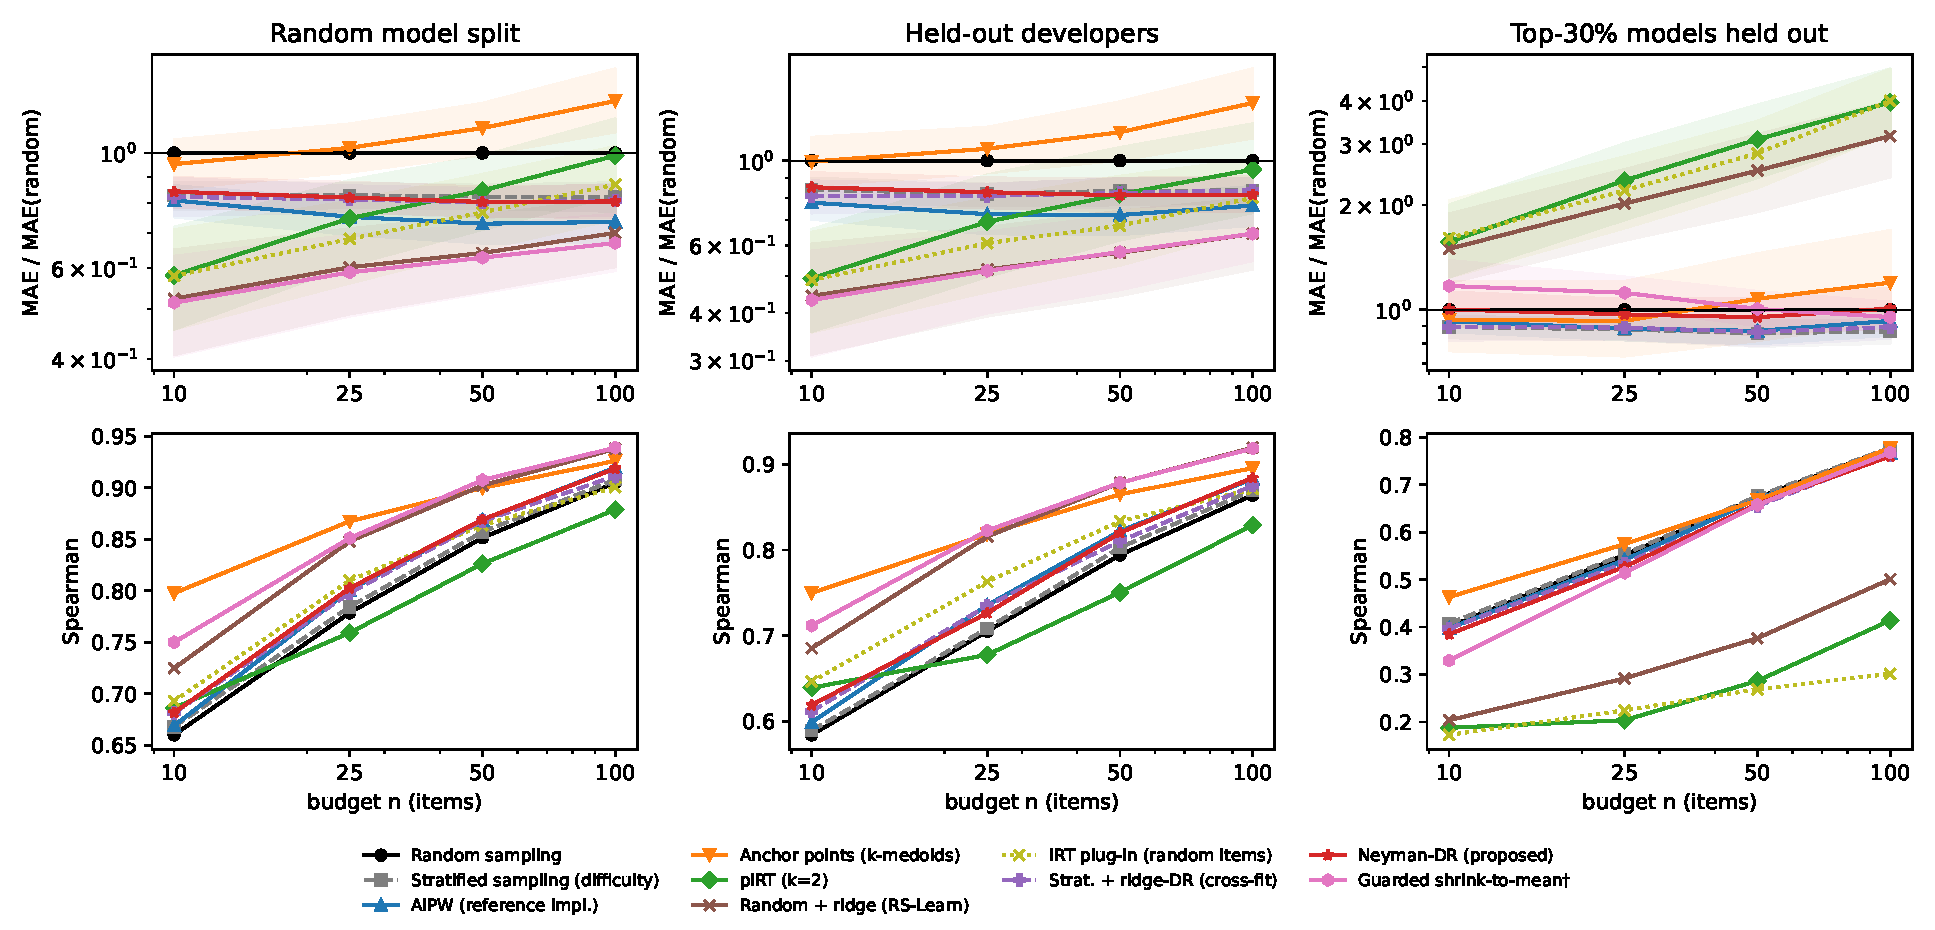
\includegraphics[width=\textwidth]{../figures/fig_budget_curves.pdf}
\caption{MAE ratio to random sampling (top, log scale, shaded 95\% bootstrap interval) and Spearman $\rho$ (bottom) versus number of items. Random sampling's absolute geometric-mean MAE is 0.10, 0.064, 0.045, 0.031 at $n=10,25,50,100$ (similar in all regimes).}
\label{fig:budget}
\end{figure}

\subsection{Source-informed prediction helps under interpolation and fails under extrapolation}
Table~\ref{tab:main} and Fig.~\ref{fig:budget} give the main picture (absolute MAE of random sampling at $n{=}50$ is $\approx0.045$).
\textbf{Interpolation and unseen developers.}
Every source-informed estimator except anchor points and pIRT has a lower MAE than random sampling at all budgets (pIRT is competitive at $n{=}10$, 0.58 on random splits, but rises to 0.99 ($k{=}2$) and 1.10 ($k{=}8$) at $n{=}100$).
The regression from coreset answers to full accuracy (RS-Learn) is best among the stage-1 methods: 0.64 [0.54, 0.76] and 0.57 [0.44, 0.74] of random's MAE at $n{=}50$, equal to the accuracy of $\approx$122 and $\approx$152 random items.
AIPW reaches 0.73 and 0.72 (equivalent to $\approx$94 and 96 items), stratified sampling on source difficulty alone 0.82 and 0.83 ($\approx$74 and 72 items), and the proposed Neyman-DR 0.80 and 0.81.
Anchor points have a worse MAE than random sampling at $n\ge25$ (1.12 at $n{=}50$, 1.26 at $n{=}100$; positive bias, Fig.~\ref{fig:bias}) but the best Spearman correlation at $n{=}10$ (0.80 vs.\ 0.66 for random sampling), so they are better at ranking than at estimating levels.
The advantage of learned predictors shrinks with budget (RS-Learn: 0.52 at $n{=}10$, 0.70 at $n{=}100$ on random splits), because sampling noise decays while model misfit does not.
\textbf{Extrapolation.}
When all targets are stronger than every source, RS-Learn, IRT plug-in and pIRT are 2.5, 2.8 and 3.1 times \emph{worse} than random sampling at $n{=}50$ (Spearman 0.38, 0.27, 0.29 vs.\ 0.67), and this gets worse with more items (RS-Learn 3.2$\times$ at $n{=}100$), because they are biased downward by 0.12--0.15 accuracy points (Fig.~\ref{fig:bias}): they shrink toward the sources' range.
Only methods with a design-unbiased component stay near random sampling: stratified sampling 0.86 [0.78, 0.93], AIPW 0.87 [0.80, 0.95], stratified ridge-DR 0.86 [0.79, 0.94]; the other estimators are statistically indistinguishable from random sampling (Neyman-DR 0.95 [0.85, 1.08]; anchors 1.08 [0.81, 1.45]).
\emph{Nothing we ran improves on difficulty-stratified sampling by more than noise under extrapolation}, and stratified sampling beats random sampling in 13/13 (interp), 7/7 (org) and 12/13 (extrap) benchmarks (Holm-adjusted $p<0.02$ for interp and extrap; with only 7 benchmarks, the smallest attainable two-sided Wilcoxon $p$ is 0.016, so Holm-adjusted org tests cannot reach 0.05; Table~\ref{app:signif}, Appendix).

\begin{figure}[t]
\centering
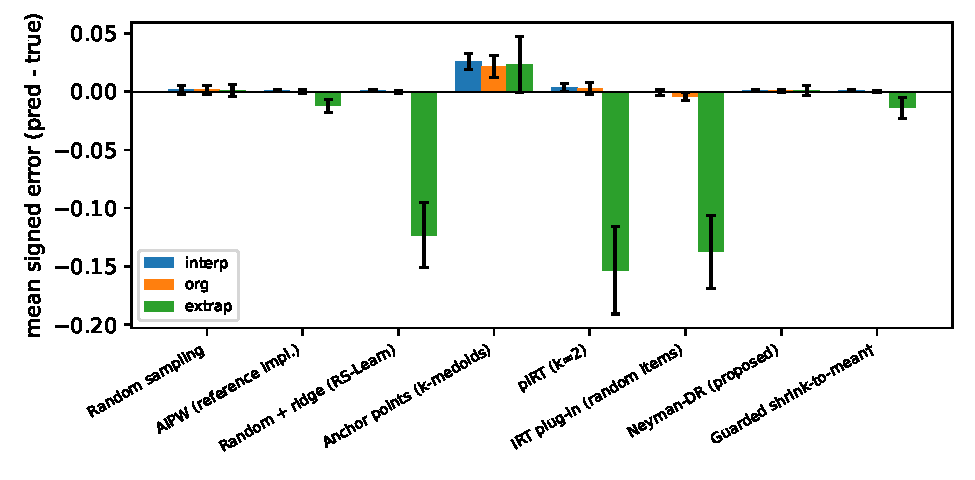
\includegraphics[width=0.62\textwidth]{../figures/fig_bias.pdf}
\caption{Mean signed error (prediction $-$ truth) at $n{=}50$, averaged over target models, seeds, and benchmarks; error bars: $\pm1.96$ s.e.\ over benchmarks. Estimators without a design-unbiased component (RS-Learn, pIRT, IRT plug-in) are strongly biased downward when targets are stronger than all sources.}
\label{fig:bias}
\end{figure}

\subsection{Design versus estimator, and the proposed Neyman-DR}
\begin{table}[t]
\centering\small
\caption{Design$\times$predictor factorial at $n{=}50$: MAE ratio to random sampling (geometric mean over benchmarks; lower is better). ``is'': residual correction computed in-sample; ``cf'': cross-fitted (5 folds). Neyman-DR (proposed) is Neyman-PPS $+$ latent $+$ cf. Intervals: \texttt{results/tables/grid\_*.csv}.}
\label{tab:grid}
\setlength{\tabcolsep}{4pt}
\begin{tabular}{ll cc cc cc}
\toprule
 & & \multicolumn{2}{c}{ridge predictor} & \multicolumn{2}{c}{latent (IRT) predictor} & \multicolumn{2}{c}{kNN predictor}\\
\cmidrule(lr){3-4}\cmidrule(lr){5-6}\cmidrule(lr){7-8}
Regime & Design & is & cf & is & cf & is & cf\\
\midrule
\multirow{3}{*}{Random split} & Uniform & 0.730 & 0.814 & 0.788 & 0.848 & 0.727 & 0.844 \\
 & Stratified & 0.712 & 0.803 & 0.782 & 0.838 & 0.722 & 0.835 \\
 & Neyman-PPS & 0.720 & 0.772 & 0.754 & 0.804 & 0.703 & 0.799 \\
\midrule
\multirow{3}{*}{Held-out developers} & Uniform & 0.721 & 0.828 & 0.801 & 0.861 & 0.737 & 0.861 \\
 & Stratified & 0.712 & 0.823 & 0.790 & 0.845 & 0.727 & 0.868 \\
 & Neyman-PPS & 0.717 & 0.787 & 0.760 & 0.812 & 0.704 & 0.818 \\
\midrule
\multirow{3}{*}{Top-30\% held out} & Uniform & 0.864 & 0.883 & 0.890 & 0.976 & 0.883 & 0.926 \\
 & Stratified & 0.839 & 0.863 & 0.850 & 0.944 & 0.856 & 0.879 \\
 & Neyman-PPS & 0.907 & 0.929 & 0.899 & 0.952 & 0.925 & 0.943 \\
\bottomrule
\end{tabular}

\end{table}
Table~\ref{tab:grid} separates design from estimator.
\textbf{Design effect.}
With the same predictor and cross-fitting, Neyman-PPS sampling reduces MAE relative to uniform sampling by 5\% under interpolation (latent: 0.948, 11/13 benchmarks, Holm $p=0.024$; ridge: 0.949, 12/13, $p=0.007$) and by a similar 5\% for held-out developers (7/7 benchmarks, but Holm $p=0.22$ because only 7 benchmarks are available).
Under extrapolation there is no gain (latent 0.98, $p=1$) or a loss (ridge 1.05, $p=0.84$).
Stratified sampling is statistically indistinguishable from uniform sampling as a design for the ridge DR estimator (0.986, $p=0.49$ under interpolation).
Ablations (Table~\ref{tab:abl}, seeds 0--9; same-design sampling noise is about $\pm0.03$, as seen from $\gamma{=}1$ vs.\ uniform) show that removing the defensive uniform component ($\gamma{=}0$) gives the largest interpolation gain (0.77) but the worst extrapolation result (1.01, worse than random sampling), consistent with residual variances learned on weak models misallocating items for strong targets; increasing the latent dimension to $k{=}8$ hurts everywhere (0.90 interp, 1.07 extrap) because 50 items cannot identify a high-dimensional ability.
\textbf{Estimator effect.}
Cross-fitting costs accuracy: in-sample ridge-DR is 0.73 vs.\ 0.81 cross-fitted under interpolation, and 0.86 vs.\ 0.88 under extrapolation; our a priori choice of cross-fitting was therefore suboptimal on average, although the in-sample estimator has no guarantee (its mean signed error is small in these data, Fig.~\ref{fig:bias}, AIPW ref.).
\textbf{Verdict on Neyman-DR.}
Neyman-DR is better than random sampling under interpolation (0.80 [0.75, 0.86]) but significantly worse than the AIPW reference (ratio 1.10, 1/13 wins, Holm $p=0.007$), much worse than RS-Learn, and not better than random sampling under extrapolation (0.95 [0.85, 1.08]).
The design effect is real but small relative to the estimator effect, so the central hypothesis---that a variance-optimal design plus a design-unbiased estimator would dominate existing methods---is not supported.

\begin{table}[t]
\centering\small
\caption{Ablations of the proposed method at $n{=}50$, cross-fitted latent estimator, MAE ratio to random sampling [95\% CI]; seeds 0--9 only ($k{=}1,4$ were fitted only for these seeds), so intervals are wider than in Table~\ref{tab:main}.}
\label{tab:abl}
\setlength{\tabcolsep}{4pt}
\begin{tabular}{l ccc}
\toprule
Variant & Random split & Held-out developers & Top-30\% held out\\
\midrule
Random sampling & 1.00 {\scriptsize[1.00,1.00]} & 1.00 {\scriptsize[1.00,1.00]} & 1.00 {\scriptsize[1.00,1.00]} \\
Uniform, $k{=}2$ & 0.83 {\scriptsize[0.75,0.92]} & 0.84 {\scriptsize[0.73,0.95]} & 0.91 {\scriptsize[0.78,1.05]} \\
Neyman-PPS $\gamma{=}0.3$, $k{=}2$ (default) & 0.81 {\scriptsize[0.73,0.90]} & 0.78 {\scriptsize[0.67,0.90]} & 0.94 {\scriptsize[0.81,1.09]} \\
Neyman-PPS $\gamma{=}0$ & 0.77 {\scriptsize[0.69,0.86]} & 0.79 {\scriptsize[0.68,0.93]} & 1.01 {\scriptsize[0.85,1.26]} \\
Neyman-PPS $\gamma{=}0.6$ & 0.79 {\scriptsize[0.71,0.88]} & 0.81 {\scriptsize[0.69,0.93]} & 0.90 {\scriptsize[0.76,1.05]} \\
$\gamma{=}1$ (uniform probabilities, systematic draw) & 0.86 {\scriptsize[0.77,0.96]} & 0.81 {\scriptsize[0.70,0.93]} & 0.93 {\scriptsize[0.81,1.06]} \\
Uniform, $k{=}1$ & 0.80 {\scriptsize[0.72,0.89]} & 0.79 {\scriptsize[0.69,0.90]} & 0.87 {\scriptsize[0.76,1.00]} \\
Neyman-PPS, $k{=}1$ & 0.79 {\scriptsize[0.72,0.88]} & 0.77 {\scriptsize[0.67,0.88]} & 0.90 {\scriptsize[0.76,1.05]} \\
Uniform, $k{=}4$ & 0.87 {\scriptsize[0.77,0.98]} & 0.88 {\scriptsize[0.76,1.04]} & 0.98 {\scriptsize[0.85,1.16]} \\
Neyman-PPS, $k{=}4$ & 0.82 {\scriptsize[0.74,0.90]} & 0.80 {\scriptsize[0.69,0.92]} & 0.98 {\scriptsize[0.83,1.17]} \\
Uniform, $k{=}8$ & 0.97 {\scriptsize[0.87,1.09]} & 0.96 {\scriptsize[0.83,1.13]} & 1.07 {\scriptsize[0.90,1.23]} \\
Neyman-PPS, $k{=}8$ & 0.90 {\scriptsize[0.82,1.00]} & 0.85 {\scriptsize[0.73,0.98]} & 1.07 {\scriptsize[0.92,1.24]} \\
\bottomrule
\end{tabular}

\end{table}

\subsection{Post hoc: regression shrunk toward the unbiased mean, with a range guard}
\label{sec:posthoc}
Stage-1 results suggested two things: learned model-level regression is strongest under interpolation, and its extrapolation failure comes from shrinking toward the source mean.
We therefore added, \emph{after} seeing stage-1 results and clearly separated in code (\texttt{run\_stage2.py}), four variants on difficulty-stratified coresets: (a) regression on coreset answers shrunk toward the design-unbiased mean (ridge on the residual full accuracy $-$ coreset mean, then add the coreset mean back), (b) RS-Learn on the same coreset, (c) a 1-D linear calibration of the coreset mean, (d) a \emph{guarded} version of (a) that falls back to the coreset mean if the target's coreset accuracy lies outside the range of the sources' coreset accuracies (no tuned constant).
Under interpolation (a) and (d) match or slightly beat RS-Learn (0.62/0.63 vs.\ 0.64; $n{=}50$) and beat stratified sampling in 13/13 benchmarks for (d) (ratio 0.76, Holm $p=0.003$).
Shrinking toward the unbiased mean reduces the extrapolation damage (2.52 $\to$ 1.39) but does not remove it, and the 1-D calibration is similarly unsafe (1.40); the guard brings extrapolation to 1.01 [0.90, 1.13] but is still 18\% worse than plain stratified sampling (stratified sampling is better in 13/13 benchmarks, Holm $p=0.003$) because some in-range targets are still mis-predicted, and the guard needs the target's coreset accuracy, not its true accuracy, to detect shift, which is noisy at small $n$.
These variants were selected after looking at the same benchmarks; they are hypotheses, not confirmed results.

\section{Discussion and limitations}
\textbf{What the evidence supports.}
(1) When targets are surrounded by source models (random splits, unseen developers), source-informed estimators other than anchors match the MAE of 72--152 random items at $n{=}50$ (1.4--3$\times$ fewer items), with learned regression best; the gain shrinks with budget.
(2) When targets exceed the sources' range, estimators lacking a design-unbiased component are 2.5--3.1$\times$ worse than random sampling, and the cheapest protection (stratified sampling on source difficulty, or AIPW) caps the gain at about 14\%.
(3) A variance-optimal sampling design gives only a $\sim$5\% error reduction on top of a given estimator, and only when shift is mild.
\textbf{What it does not support.} We have no evidence that Neyman-DR is a practical improvement, and our post hoc estimators are untested out-of-sample.
\textbf{Limitations.}
(i) Only binary item matrices from two leaderboard families; the 7 Open LLM benchmarks share the same model population, so benchmarks are not independent, and bootstrap and Wilcoxon intervals treat them as exchangeable.
(ii) The model population has near-duplicates (4--16\% of Open LLM model rows are exact duplicates of another row within a benchmark, Appendix Table~\ref{tab:data}), favoring interpolation.
(iii) The extrapolation split is one fixed partition per benchmark, so its intervals reflect coreset randomness and benchmark heterogeneity, not model-split uncertainty; the three regimes are not exhaustive (\eg\ no temporal split).
(iv) IRT components are our own MAP fits (no hierarchical priors, 2 or 8 dimensions, 150 L-BFGS iterations), not the original implementations; pIRT may be disadvantaged.
(v) We did not run metabench, assessor-based~\citep{pacchiardi2024100}, active~\citep{li2025active} or adaptive~\citep{balkir2026adaptive} methods, nor the reference repository's PCA, lasso, double-optimize and sort-and-search methods.
(vi) Defaults ($k{=}2$, $\gamma{=}0.3$, $\alpha{=}10$, 5 folds, $K{=}10$ neighbours) were fixed in advance and not tuned; ablations cover only $k$ and $\gamma$, and on 10 seeds.
(vii) The anchor-point $k$-means variant in pIRT may select the same item for two clusters (not merged in the stage-1 code; negligible effect expected, not quantified).
(viii) The ground truth is each target's observed full-benchmark accuracy; item-level noise and benchmark contamination are not modeled.

\paragraph{Reproducibility statement.}
Code, exact commands, seeds, library versions and a table-to-script map are in the supplementary \texttt{README.md}; data are the public files at commit \texttt{55faff4} of the cited repository; the main grid took about 3.5 h on a shared CPU machine (Sec.~\ref{sec:exp}, Appendix~\ref{app:repro}).

\paragraph{Ethics statement.}
The work uses public, aggregated item-level outcomes of public models; it involves no human subjects. A risk is over-reliance on small coresets to certify models; our results show that learned predictors can be biased by large margins for models stronger than those seen.

\subsection*{AI use statement}
The research was carried out end to end by an autonomous AI research agent (an LLM-based coding agent) running unattended: it designed the study, wrote the code, executed the experiments, performed the analysis and drafted this paper; no human author checked the code line by line. Verification steps included: shared-coreset consistency checks between the two code stages (identical errors for random sampling and RS-Learn, max difference $0$), pilot runs, and re-generation of every table and figure from \texttt{results/main.csv} and \texttt{results/stage2.csv}. All claims, including limitations, are the agent's responsibility; the agent's citations were checked for existence via the arXiv API (titles and dates) or are standard textbooks, and papers were characterized only from the abstract-level descriptions provided with the task and, for the data repository, from its README and source code.

\bibliography{refs}
\bibliographystyle{iclr2027_conference}

\appendix
\section{Additional tables}
\label{app:tables}
\begin{table}[h]
\centering\scriptsize
\caption{Datasets (after loading the \texttt{.jbl} matrices at commit \texttt{55faff4}). \emph{sd}: standard deviation of model accuracies; \emph{const.}: fraction of items answered identically by all models; \emph{dup.}: fraction of model rows that duplicate another row.}
\label{tab:data}
\begin{tabular}{llrrrrrrr}
\toprule
Dataset & Family & Models & Items & Mean acc. & sd & Range & const. & dup.\\
\midrule
ifeval & OpenLLM & 448 & 541 & 0.333 & 0.204 & 0.04--0.88 & 0.013 & 0.047 \\
openllm\_math & OpenLLM & 447 & 894 & 0.051 & 0.068 & 0.00--0.36 & 0.133 & 0.161 \\
mmlu\_pro & OpenLLM & 448 & 12032 & 0.281 & 0.129 & 0.10--0.60 & 0.000 & 0.051 \\
arc\_challenge & OpenLLM & 218 & 1172 & 0.522 & 0.129 & 0.20--0.75 & 0.027 & 0.041 \\
bbh & OpenLLM & 446 & 5761 & 0.447 & 0.116 & 0.24--0.75 & 0.000 & 0.047 \\
gpqa & OpenLLM & 447 & 1192 & 0.289 & 0.038 & 0.23--0.44 & 0.000 & 0.051 \\
musr & OpenLLM & 448 & 756 & 0.399 & 0.041 & 0.32--0.54 & 0.013 & 0.047 \\
commonsense & HELM & 83 & 500 & 0.823 & 0.173 & 0.22--0.97 & 0.000 & 0.012 \\
gsm & HELM & 83 & 1000 & 0.657 & 0.249 & 0.03--0.96 & 0.003 & 0.000 \\
legalbench & HELM & 79 & 2047 & 0.533 & 0.106 & 0.23--0.70 & 0.026 & 0.000 \\
math & HELM & 83 & 437 & 0.568 & 0.274 & 0.03--0.93 & 0.002 & 0.000 \\
med\_qa & HELM & 83 & 1000 & 0.594 & 0.164 & 0.21--0.87 & 0.002 & 0.012 \\
mmlu & HELM & 83 & 567 & 0.613 & 0.124 & 0.23--0.81 & 0.002 & 0.012 \\
\bottomrule
\end{tabular}

\end{table}

\begin{table}[h]
\centering\scriptsize
\caption{Per-benchmark MAE ratio to random sampling at $n{=}50$ (mean over 30 seeds). Blocks: random split, held-out developers (Open LLM only), top-30\% held out. Columns: stratified, RS-Learn, AIPW (ref.), anchors, pIRT ($k{=}2$), strat.+ridge-DR (cf), Neyman-DR, guarded shrink-to-mean$^\dagger$.}
\label{tab:perds}
\setlength{\tabcolsep}{3pt}
\begin{tabular}{l cccccccc}
\toprule
Benchmark & Strat & RS-L & AIPW & Anch & pIRT & S+rDR & N-DR & Guard\\
\midrule
\multicolumn{9}{l}{\emph{Random split}}\\
arc\_challenge & 0.75 & 0.61 & 0.63 & 1.31 & 0.89 & 0.74 & 0.67 & 0.58 \\
bbh & 0.86 & 0.51 & 0.68 & 1.20 & 0.75 & 0.79 & 0.83 & 0.56 \\
commonsense & 0.84 & 0.83 & 0.84 & 1.14 & 1.05 & 0.83 & 0.88 & 0.77 \\
gpqa & 0.89 & 0.34 & 0.77 & 0.87 & 0.50 & 0.82 & 0.87 & 0.35 \\
gsm & 0.82 & 0.88 & 0.84 & 1.18 & 0.91 & 0.83 & 0.81 & 0.80 \\
ifeval & 0.87 & 0.73 & 0.79 & 1.67 & 0.76 & 0.84 & 0.81 & 0.74 \\
legalbench & 0.75 & 0.63 & 0.63 & 0.88 & 1.02 & 0.67 & 0.70 & 0.59 \\
math & 0.80 & 0.85 & 0.84 & 1.26 & 1.03 & 0.83 & 0.85 & 0.77 \\
med\_qa & 0.83 & 0.78 & 0.74 & 0.90 & 1.12 & 0.83 & 0.82 & 0.75 \\
mmlu & 0.80 & 0.69 & 0.73 & 0.89 & 0.79 & 0.83 & 0.78 & 0.70 \\
mmlu\_pro & 0.86 & 0.61 & 0.72 & 1.28 & 1.00 & 0.81 & 0.83 & 0.64 \\
musr & 0.76 & 0.34 & 0.51 & 0.90 & 0.43 & 0.70 & 0.70 & 0.35 \\
openllm\_math & 0.90 & 0.91 & 0.88 & 1.35 & 1.19 & 0.95 & 0.94 & 0.85 \\
\midrule
\multicolumn{9}{l}{\emph{Held-out developers}}\\
arc\_challenge & 0.69 & 0.62 & 0.62 & 1.24 & 0.83 & 0.69 & 0.66 & 0.57 \\
bbh & 0.84 & 0.54 & 0.70 & 1.18 & 0.91 & 0.81 & 0.82 & 0.58 \\
gpqa & 0.91 & 0.37 & 0.80 & 0.86 & 0.54 & 0.87 & 0.88 & 0.38 \\
ifeval & 0.89 & 0.76 & 0.80 & 1.74 & 0.83 & 0.89 & 0.86 & 0.77 \\
mmlu\_pro & 0.87 & 0.66 & 0.75 & 1.25 & 1.18 & 0.85 & 0.85 & 0.67 \\
musr & 0.75 & 0.35 & 0.53 & 0.90 & 0.44 & 0.73 & 0.69 & 0.38 \\
openllm\_math & 0.90 & 0.96 & 0.90 & 1.33 & 1.38 & 0.96 & 0.97 & 0.87 \\
\midrule
\multicolumn{9}{l}{\emph{Top-30\% held out}}\\
arc\_challenge & 0.75 & 2.10 & 0.95 & 1.35 & 4.56 & 0.78 & 0.83 & 0.94 \\
bbh & 0.97 & 2.96 & 0.86 & 1.59 & 3.48 & 0.96 & 0.95 & 1.40 \\
commonsense & 0.93 & 3.17 & 0.96 & 0.67 & 4.59 & 1.00 & 0.91 & 1.24 \\
gpqa & 0.90 & 1.23 & 0.89 & 0.85 & 1.42 & 0.91 & 0.91 & 1.17 \\
gsm & 0.85 & 3.18 & 0.94 & 1.31 & 2.84 & 0.88 & 1.01 & 0.89 \\
ifeval & 0.96 & 4.78 & 0.92 & 1.27 & 6.37 & 0.93 & 1.45 & 0.97 \\
legalbench & 0.67 & 1.36 & 0.67 & 0.61 & 2.59 & 0.64 & 0.70 & 0.78 \\
math & 0.84 & 2.97 & 0.90 & 0.94 & 3.35 & 0.88 & 1.09 & 0.85 \\
med\_qa & 0.70 & 3.83 & 0.89 & 0.66 & 4.36 & 0.75 & 0.81 & 0.77 \\
mmlu & 0.84 & 2.77 & 0.87 & 0.63 & 2.92 & 0.85 & 0.98 & 0.95 \\
mmlu\_pro & 1.08 & 3.14 & 0.92 & 1.61 & 2.78 & 1.07 & 1.05 & 1.35 \\
musr & 0.79 & 1.03 & 0.63 & 0.76 & 1.27 & 0.74 & 0.72 & 0.95 \\
openllm\_math & 0.93 & 3.20 & 0.99 & 4.28 & 3.30 & 0.95 & 1.21 & 1.05 \\
\bottomrule
\end{tabular}

\end{table}

\begin{figure}[h]
\centering
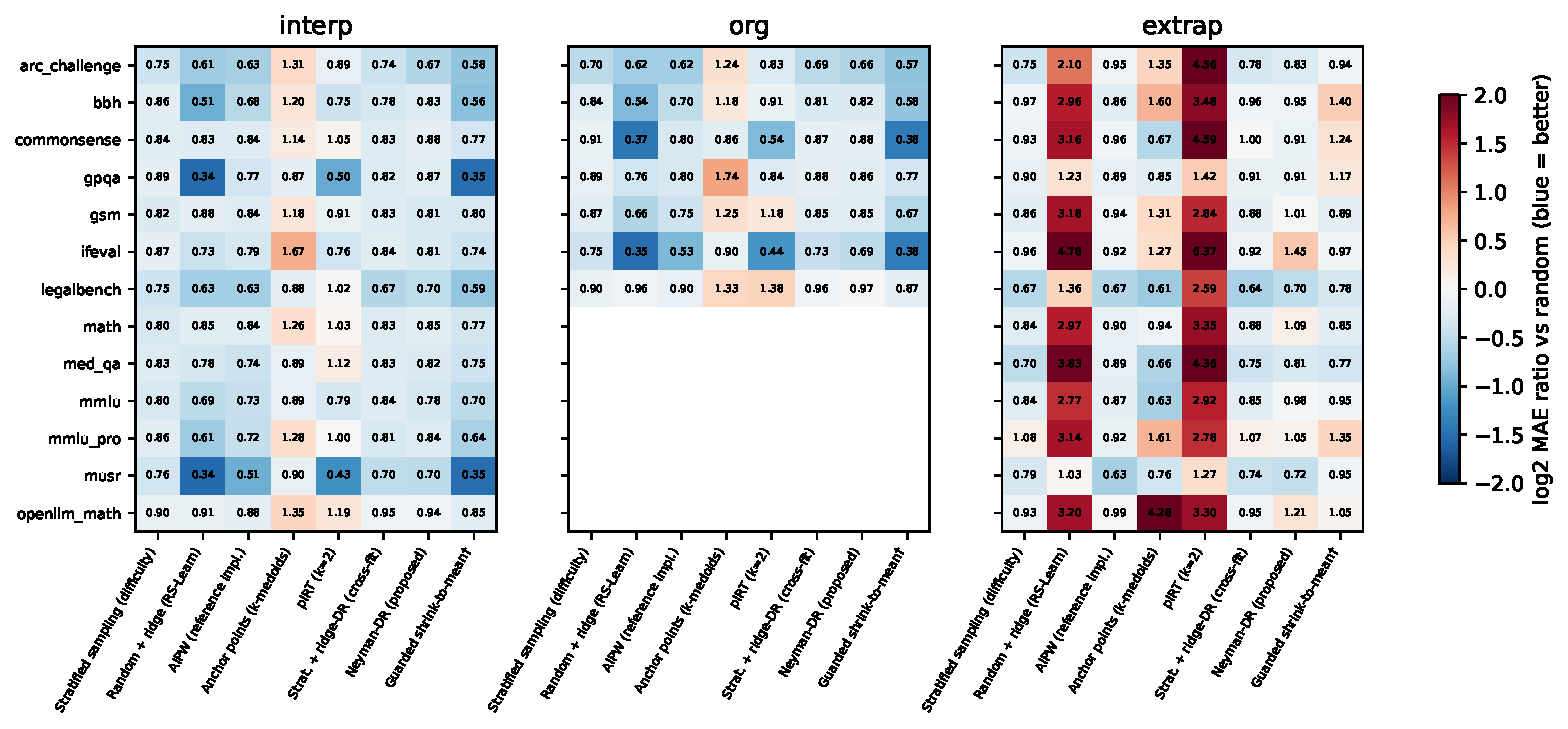
\includegraphics[width=\textwidth]{../figures/fig_heatmap.pdf}
\caption{Per-benchmark MAE ratio to random sampling at $n{=}50$ (cell text = ratio; blue = better than random).}
\end{figure}

\begin{table}[h]
\centering\scriptsize
\caption{Paired tests at $n{=}50$ (full results for all budgets: \texttt{results/tables/significance.csv}). Geometric mean ratio of seed-averaged MAE (first method / second), number of benchmarks where the first method is better, two-sided Wilcoxon signed-rank $p$ across benchmarks, and Holm-adjusted $p$ over the 14 listed pairs within each regime. The last three pairs of each block are post hoc. With 7 benchmarks the smallest attainable $p$ is 0.0156.}
\label{app:signif}
\begin{tabular}{llcccc}
\toprule
Regime & Pair & ratio & wins & $p$ & Holm $p$\\
\midrule
interp & \texttt{pps\_resid+lat\_cf} vs \texttt{random} & 0.804 & 13/13 & 0.0002 & 0.0034 \\
interp & \texttt{pps\_resid+lat\_cf} vs \texttt{aipw\_ref} & 1.102 & 1/13 & 0.0007 & 0.0066 \\
interp & \texttt{pps\_resid+lat\_cf} vs \texttt{uniform+lat\_cf} & 0.948 & 11/13 & 0.0034 & 0.0239 \\
interp & \texttt{pps\_resid+ridge\_cf} vs \texttt{uniform+ridge\_cf} & 0.949 & 12/13 & 0.0007 & 0.0066 \\
interp & \texttt{strat+ridge\_cf} vs \texttt{uniform+ridge\_cf} & 0.986 & 8/13 & 0.2439 & 0.4878 \\
interp & \texttt{aipw\_ref} vs \texttt{random} & 0.730 & 13/13 & 0.0002 & 0.0034 \\
interp & \texttt{strat\_mean} vs \texttt{random} & 0.824 & 13/13 & 0.0002 & 0.0034 \\
interp & \texttt{anchor\_w} vs \texttt{random} & 1.117 & 5/13 & 0.0398 & 0.1990 \\
interp & \texttt{pirt\_k2} vs \texttt{random} & 0.846 & 8/13 & 0.1272 & 0.3816 \\
interp & \texttt{rs\_learn} vs \texttt{random} & 0.641 & 13/13 & 0.0002 & 0.0034 \\
interp & \texttt{rs\_learn} vs \texttt{strat\_mean} & 0.778 & 10/13 & 0.0105 & 0.0630 \\
interp & \texttt{guard\_strat} vs \texttt{strat\_mean} & 0.762 & 13/13 & 0.0002 & 0.0034 \\
interp & \texttt{guard\_strat} vs \texttt{rs\_learn} & 0.979 & 7/13 & 0.2734 & 0.4878 \\
interp & \texttt{rsres\_strat} vs \texttt{rs\_learn} & 0.968 & 9/13 & 0.0942 & 0.3770 \\
\midrule
org & \texttt{pps\_resid+lat\_cf} vs \texttt{random} & 0.812 & 7/7 & 0.0156 & 0.2188 \\
org & \texttt{pps\_resid+lat\_cf} vs \texttt{aipw\_ref} & 1.126 & 0/7 & 0.0156 & 0.2188 \\
org & \texttt{pps\_resid+lat\_cf} vs \texttt{uniform+lat\_cf} & 0.943 & 7/7 & 0.0156 & 0.2188 \\
org & \texttt{pps\_resid+ridge\_cf} vs \texttt{uniform+ridge\_cf} & 0.951 & 7/7 & 0.0156 & 0.2188 \\
org & \texttt{strat+ridge\_cf} vs \texttt{uniform+ridge\_cf} & 0.994 & 3/7 & 0.8125 & 1.0000 \\
org & \texttt{aipw\_ref} vs \texttt{random} & 0.721 & 7/7 & 0.0156 & 0.2188 \\
org & \texttt{strat\_mean} vs \texttt{random} & 0.834 & 7/7 & 0.0156 & 0.2188 \\
org & \texttt{anchor\_w} vs \texttt{random} & 1.186 & 2/7 & 0.0781 & 0.3906 \\
org & \texttt{pirt\_k2} vs \texttt{random} & 0.817 & 5/7 & 0.2969 & 1.0000 \\
org & \texttt{rs\_learn} vs \texttt{random} & 0.574 & 7/7 & 0.0156 & 0.2188 \\
org & \texttt{rs\_learn} vs \texttt{strat\_mean} & 0.689 & 6/7 & 0.0312 & 0.2188 \\
org & \texttt{guard\_strat} vs \texttt{strat\_mean} & 0.692 & 7/7 & 0.0156 & 0.2188 \\
org & \texttt{guard\_strat} vs \texttt{rs\_learn} & 1.005 & 2/7 & 0.8125 & 1.0000 \\
org & \texttt{rsres\_strat} vs \texttt{rs\_learn} & 0.990 & 2/7 & 0.9375 & 1.0000 \\
\midrule
extrap & \texttt{pps\_resid+lat\_cf} vs \texttt{random} & 0.952 & 8/13 & 0.3396 & 1.0000 \\
extrap & \texttt{pps\_resid+lat\_cf} vs \texttt{aipw\_ref} & 1.095 & 3/13 & 0.0574 & 0.3442 \\
extrap & \texttt{pps\_resid+lat\_cf} vs \texttt{uniform+lat\_cf} & 0.975 & 8/13 & 0.4548 & 1.0000 \\
extrap & \texttt{pps\_resid+ridge\_cf} vs \texttt{uniform+ridge\_cf} & 1.053 & 5/13 & 0.1677 & 0.8386 \\
extrap & \texttt{strat+ridge\_cf} vs \texttt{uniform+ridge\_cf} & 0.978 & 9/13 & 0.2163 & 0.8652 \\
extrap & \texttt{aipw\_ref} vs \texttt{random} & 0.869 & 13/13 & 0.0002 & 0.0034 \\
extrap & \texttt{strat\_mean} vs \texttt{random} & 0.856 & 12/13 & 0.0024 & 0.0171 \\
extrap & \texttt{anchor\_w} vs \texttt{random} & 1.076 & 7/13 & 0.8926 & 1.0000 \\
extrap & \texttt{pirt\_k2} vs \texttt{random} & 3.097 & 0/13 & 0.0002 & 0.0034 \\
extrap & \texttt{rs\_learn} vs \texttt{random} & 2.518 & 0/13 & 0.0002 & 0.0034 \\
extrap & \texttt{rs\_learn} vs \texttt{strat\_mean} & 2.943 & 0/13 & 0.0002 & 0.0034 \\
extrap & \texttt{guard\_strat} vs \texttt{strat\_mean} & 1.176 & 0/13 & 0.0002 & 0.0034 \\
extrap & \texttt{guard\_strat} vs \texttt{rs\_learn} & 0.400 & 13/13 & 0.0002 & 0.0034 \\
extrap & \texttt{rsres\_strat} vs \texttt{rs\_learn} & 0.553 & 13/13 & 0.0002 & 0.0034 \\
\bottomrule
\end{tabular}

\end{table}

\begin{table}[h]
\centering\scriptsize
\caption{Random model split: all budgets. MAE and RMSE as ratio to random sampling, Spearman and Kendall (mean over benchmarks); 95\% bootstrap intervals in braces.}
\setlength{\tabcolsep}{3pt}
\begin{tabular}{l cccc}
\toprule
Method & MAE ratio & RMSE ratio & Spearman & Kendall\\
\midrule
\multicolumn{5}{l}{\emph{$n=10$}}\\
Random sampling & 1.000 {\scriptsize[1.000,1.000]} & 1.000 {\scriptsize[1.000,1.000]} & 0.660 {\scriptsize[0.549,0.752]} & 0.543 {\scriptsize[0.443,0.638]} \\
Stratified sampling (difficulty) & 0.828 {\scriptsize[0.778,0.878]} & 0.846 {\scriptsize[0.802,0.893]} & 0.668 {\scriptsize[0.552,0.758]} & 0.543 {\scriptsize[0.438,0.632]} \\
Random + ridge (RS-Learn) & 0.523 {\scriptsize[0.408,0.650]} & 0.538 {\scriptsize[0.432,0.660]} & 0.725 {\scriptsize[0.650,0.788]} & 0.572 {\scriptsize[0.504,0.641]} \\
AIPW (reference impl.) & 0.810 {\scriptsize[0.752,0.865]} & 0.832 {\scriptsize[0.785,0.880]} & 0.669 {\scriptsize[0.553,0.760]} & 0.530 {\scriptsize[0.428,0.624]} \\
Anchor points (k-medoids) & 0.952 {\scriptsize[0.853,1.061]} & 0.953 {\scriptsize[0.860,1.063]} & \textbf{0.798} {\scriptsize[0.729,0.852]} & \textbf{0.651} {\scriptsize[0.574,0.715]} \\
pIRT (k=2) & 0.580 {\scriptsize[0.457,0.719]} & 0.613 {\scriptsize[0.496,0.750]} & 0.686 {\scriptsize[0.613,0.754]} & 0.542 {\scriptsize[0.477,0.606]} \\
pIRT (k=8) & 0.621 {\scriptsize[0.503,0.747]} & 0.652 {\scriptsize[0.537,0.795]} & 0.677 {\scriptsize[0.575,0.747]} & 0.531 {\scriptsize[0.444,0.601]} \\
IRT plug-in (random items) & 0.579 {\scriptsize[0.456,0.711]} & 0.610 {\scriptsize[0.494,0.742]} & 0.693 {\scriptsize[0.602,0.766]} & 0.545 {\scriptsize[0.464,0.624]} \\
Uniform + latent-DR (cf) & 0.890 {\scriptsize[0.836,0.941]} & 0.907 {\scriptsize[0.864,0.955]} & 0.665 {\scriptsize[0.554,0.753]} & 0.524 {\scriptsize[0.430,0.611]} \\
Uniform + kNN-DR (cf) & 0.903 {\scriptsize[0.845,0.964]} & 0.912 {\scriptsize[0.871,0.958]} & 0.661 {\scriptsize[0.548,0.751]} & 0.520 {\scriptsize[0.425,0.612]} \\
Neyman-DR (proposed) & 0.842 {\scriptsize[0.785,0.897]} & 0.868 {\scriptsize[0.820,0.921]} & 0.682 {\scriptsize[0.573,0.759]} & 0.534 {\scriptsize[0.447,0.620]} \\
Neyman-PPS + ridge-DR (cf) & 0.858 {\scriptsize[0.800,0.917]} & 0.883 {\scriptsize[0.836,0.938]} & 0.672 {\scriptsize[0.562,0.752]} & 0.525 {\scriptsize[0.436,0.610]} \\
Strat.\ + ridge-DR (cross-fit) & 0.822 {\scriptsize[0.757,0.894]} & 0.842 {\scriptsize[0.789,0.905]} & 0.681 {\scriptsize[0.573,0.763]} & 0.535 {\scriptsize[0.441,0.618]} \\
Shrink-to-mean regression$^\dagger$ & \textbf{0.506} {\scriptsize[0.397,0.626]} & \textbf{0.522} {\scriptsize[0.422,0.641]} & 0.750 {\scriptsize[0.683,0.804]} & 0.593 {\scriptsize[0.528,0.653]} \\
Guarded shrink-to-mean$^\dagger$ & 0.514 {\scriptsize[0.405,0.632]} & 0.541 {\scriptsize[0.443,0.653]} & 0.750 {\scriptsize[0.682,0.804]} & 0.593 {\scriptsize[0.528,0.652]} \\
RS-Learn on strat.\ coreset$^\dagger$ & 0.507 {\scriptsize[0.399,0.628]} & 0.523 {\scriptsize[0.422,0.642]} & 0.749 {\scriptsize[0.682,0.802]} & 0.591 {\scriptsize[0.526,0.651]} \\
1-D calibration$^\dagger$ & 0.563 {\scriptsize[0.446,0.685]} & 0.571 {\scriptsize[0.466,0.694]} & 0.669 {\scriptsize[0.554,0.758]} & 0.544 {\scriptsize[0.440,0.633]} \\
\midrule
\multicolumn{5}{l}{\emph{$n=25$}}\\
Random sampling & 1.000 {\scriptsize[1.000,1.000]} & 1.000 {\scriptsize[1.000,1.000]} & 0.779 {\scriptsize[0.671,0.869]} & 0.651 {\scriptsize[0.538,0.738]} \\
Stratified sampling (difficulty) & 0.828 {\scriptsize[0.784,0.874]} & 0.844 {\scriptsize[0.804,0.887]} & 0.784 {\scriptsize[0.687,0.864]} & 0.646 {\scriptsize[0.540,0.729]} \\
Random + ridge (RS-Learn) & 0.601 {\scriptsize[0.489,0.714]} & 0.618 {\scriptsize[0.507,0.736]} & 0.848 {\scriptsize[0.794,0.893]} & 0.694 {\scriptsize[0.630,0.749]} \\
AIPW (reference impl.) & 0.753 {\scriptsize[0.695,0.810]} & 0.771 {\scriptsize[0.720,0.828]} & 0.801 {\scriptsize[0.701,0.881]} & 0.653 {\scriptsize[0.548,0.732]} \\
Anchor points (k-medoids) & 1.023 {\scriptsize[0.919,1.138]} & 1.022 {\scriptsize[0.918,1.144]} & \textbf{0.867} {\scriptsize[0.810,0.916]} & \textbf{0.724} {\scriptsize[0.654,0.782]} \\
pIRT (k=2) & 0.748 {\scriptsize[0.607,0.885]} & 0.828 {\scriptsize[0.672,0.987]} & 0.759 {\scriptsize[0.681,0.829]} & 0.614 {\scriptsize[0.534,0.689]} \\
pIRT (k=8) & 0.810 {\scriptsize[0.669,0.966]} & 0.869 {\scriptsize[0.717,1.061]} & 0.763 {\scriptsize[0.663,0.838]} & 0.606 {\scriptsize[0.510,0.676]} \\
IRT plug-in (random items) & 0.682 {\scriptsize[0.560,0.807]} & 0.730 {\scriptsize[0.607,0.858]} & 0.810 {\scriptsize[0.739,0.872]} & 0.660 {\scriptsize[0.579,0.727]} \\
Uniform + latent-DR (cf) & 0.875 {\scriptsize[0.826,0.924]} & 0.893 {\scriptsize[0.848,0.944]} & 0.790 {\scriptsize[0.693,0.872]} & 0.640 {\scriptsize[0.535,0.721]} \\
Uniform + kNN-DR (cf) & 0.876 {\scriptsize[0.824,0.931]} & 0.890 {\scriptsize[0.847,0.939]} & 0.785 {\scriptsize[0.685,0.867]} & 0.635 {\scriptsize[0.529,0.717]} \\
Neyman-DR (proposed) & 0.820 {\scriptsize[0.769,0.878]} & 0.851 {\scriptsize[0.794,0.908]} & 0.802 {\scriptsize[0.701,0.881]} & 0.653 {\scriptsize[0.548,0.731]} \\
Neyman-PPS + ridge-DR (cf) & 0.796 {\scriptsize[0.742,0.852]} & 0.822 {\scriptsize[0.768,0.878]} & 0.800 {\scriptsize[0.701,0.879]} & 0.650 {\scriptsize[0.546,0.728]} \\
Strat.\ + ridge-DR (cross-fit) & 0.813 {\scriptsize[0.769,0.864]} & 0.832 {\scriptsize[0.789,0.885]} & 0.798 {\scriptsize[0.712,0.869]} & 0.646 {\scriptsize[0.551,0.721]} \\
Shrink-to-mean regression$^\dagger$ & \textbf{0.580} {\scriptsize[0.476,0.689]} & \textbf{0.599} {\scriptsize[0.492,0.705]} & 0.851 {\scriptsize[0.804,0.895]} & 0.698 {\scriptsize[0.637,0.751]} \\
Guarded shrink-to-mean$^\dagger$ & 0.588 {\scriptsize[0.484,0.694]} & 0.614 {\scriptsize[0.512,0.717]} & 0.851 {\scriptsize[0.803,0.895]} & 0.697 {\scriptsize[0.636,0.751]} \\
RS-Learn on strat.\ coreset$^\dagger$ & 0.593 {\scriptsize[0.481,0.711]} & 0.611 {\scriptsize[0.497,0.727]} & 0.853 {\scriptsize[0.806,0.896]} & 0.699 {\scriptsize[0.638,0.751]} \\
1-D calibration$^\dagger$ & 0.663 {\scriptsize[0.560,0.757]} & 0.675 {\scriptsize[0.572,0.771]} & 0.784 {\scriptsize[0.687,0.864]} & 0.646 {\scriptsize[0.540,0.729]} \\
\midrule
\multicolumn{5}{l}{\emph{$n=50$}}\\
Random sampling & 1.000 {\scriptsize[1.000,1.000]} & 1.000 {\scriptsize[1.000,1.000]} & 0.851 {\scriptsize[0.761,0.921]} & 0.728 {\scriptsize[0.636,0.803]} \\
Stratified sampling (difficulty) & 0.824 {\scriptsize[0.781,0.867]} & 0.838 {\scriptsize[0.799,0.877]} & 0.857 {\scriptsize[0.776,0.921]} & 0.725 {\scriptsize[0.636,0.797]} \\
Random + ridge (RS-Learn) & 0.641 {\scriptsize[0.541,0.757]} & 0.660 {\scriptsize[0.555,0.772]} & 0.902 {\scriptsize[0.867,0.934]} & 0.763 {\scriptsize[0.711,0.808]} \\
AIPW (reference impl.) & 0.730 {\scriptsize[0.670,0.793]} & 0.748 {\scriptsize[0.689,0.804]} & 0.868 {\scriptsize[0.794,0.927]} & 0.731 {\scriptsize[0.650,0.796]} \\
Anchor points (k-medoids) & 1.117 {\scriptsize[0.992,1.248]} & 1.122 {\scriptsize[0.997,1.259]} & 0.900 {\scriptsize[0.855,0.939]} & 0.767 {\scriptsize[0.700,0.821]} \\
pIRT (k=2) & 0.846 {\scriptsize[0.712,0.987]} & 0.974 {\scriptsize[0.794,1.156]} & 0.826 {\scriptsize[0.755,0.889]} & 0.693 {\scriptsize[0.613,0.763]} \\
pIRT (k=8) & 0.966 {\scriptsize[0.786,1.155]} & 1.061 {\scriptsize[0.867,1.297]} & 0.813 {\scriptsize[0.728,0.880]} & 0.666 {\scriptsize[0.580,0.732]} \\
IRT plug-in (random items) & 0.768 {\scriptsize[0.651,0.909]} & 0.835 {\scriptsize[0.684,1.018]} & 0.864 {\scriptsize[0.809,0.915]} & 0.724 {\scriptsize[0.649,0.788]} \\
Uniform + latent-DR (cf) & 0.848 {\scriptsize[0.792,0.918]} & 0.875 {\scriptsize[0.817,0.947]} & 0.857 {\scriptsize[0.778,0.920]} & 0.718 {\scriptsize[0.631,0.788]} \\
Uniform + kNN-DR (cf) & 0.844 {\scriptsize[0.787,0.906]} & 0.863 {\scriptsize[0.809,0.914]} & 0.858 {\scriptsize[0.782,0.919]} & 0.718 {\scriptsize[0.633,0.785]} \\
Neyman-DR (proposed) & 0.804 {\scriptsize[0.755,0.860]} & 0.836 {\scriptsize[0.778,0.898]} & 0.869 {\scriptsize[0.796,0.929]} & 0.731 {\scriptsize[0.645,0.799]} \\
Neyman-PPS + ridge-DR (cf) & 0.772 {\scriptsize[0.727,0.821]} & 0.798 {\scriptsize[0.748,0.849]} & 0.869 {\scriptsize[0.793,0.929]} & 0.731 {\scriptsize[0.643,0.799]} \\
Strat.\ + ridge-DR (cross-fit) & 0.803 {\scriptsize[0.752,0.854]} & 0.824 {\scriptsize[0.778,0.871]} & 0.868 {\scriptsize[0.796,0.924]} & 0.727 {\scriptsize[0.648,0.794]} \\
Shrink-to-mean regression$^\dagger$ & \textbf{0.620} {\scriptsize[0.528,0.719]} & \textbf{0.640} {\scriptsize[0.542,0.737]} & \textbf{0.907} {\scriptsize[0.873,0.937]} & \textbf{0.771} {\scriptsize[0.721,0.815]} \\
Guarded shrink-to-mean$^\dagger$ & 0.628 {\scriptsize[0.537,0.725]} & 0.652 {\scriptsize[0.559,0.744]} & 0.907 {\scriptsize[0.873,0.937]} & 0.771 {\scriptsize[0.721,0.815]} \\
RS-Learn on strat.\ coreset$^\dagger$ & 0.636 {\scriptsize[0.534,0.750]} & 0.658 {\scriptsize[0.551,0.772]} & 0.907 {\scriptsize[0.874,0.937]} & 0.770 {\scriptsize[0.722,0.814]} \\
1-D calibration$^\dagger$ & 0.717 {\scriptsize[0.636,0.797]} & 0.732 {\scriptsize[0.645,0.811]} & 0.857 {\scriptsize[0.776,0.921]} & 0.725 {\scriptsize[0.636,0.797]} \\
\midrule
\multicolumn{5}{l}{\emph{$n=100$}}\\
Random sampling & 1.000 {\scriptsize[1.000,1.000]} & 1.000 {\scriptsize[1.000,1.000]} & 0.905 {\scriptsize[0.837,0.955]} & 0.794 {\scriptsize[0.718,0.857]} \\
Stratified sampling (difficulty) & 0.822 {\scriptsize[0.771,0.876]} & 0.838 {\scriptsize[0.789,0.881]} & 0.908 {\scriptsize[0.842,0.956]} & 0.792 {\scriptsize[0.716,0.855]} \\
Random + ridge (RS-Learn) & 0.701 {\scriptsize[0.603,0.818]} & 0.723 {\scriptsize[0.622,0.831]} & 0.938 {\scriptsize[0.912,0.960]} & 0.820 {\scriptsize[0.778,0.858]} \\
AIPW (reference impl.) & 0.736 {\scriptsize[0.672,0.805]} & 0.755 {\scriptsize[0.699,0.814]} & 0.920 {\scriptsize[0.866,0.958]} & 0.802 {\scriptsize[0.736,0.857]} \\
Anchor points (k-medoids) & 1.261 {\scriptsize[1.098,1.454]} & 1.271 {\scriptsize[1.097,1.464]} & 0.926 {\scriptsize[0.889,0.956]} & 0.807 {\scriptsize[0.753,0.852]} \\
pIRT (k=2) & 0.988 {\scriptsize[0.829,1.164]} & 1.183 {\scriptsize[0.956,1.454]} & 0.879 {\scriptsize[0.828,0.926]} & 0.757 {\scriptsize[0.691,0.816]} \\
pIRT (k=8) & 1.096 {\scriptsize[0.905,1.328]} & 1.266 {\scriptsize[1.000,1.562]} & 0.877 {\scriptsize[0.809,0.934]} & 0.750 {\scriptsize[0.673,0.813]} \\
IRT plug-in (random items) & 0.870 {\scriptsize[0.745,1.029]} & 0.970 {\scriptsize[0.807,1.173]} & 0.900 {\scriptsize[0.850,0.944]} & 0.780 {\scriptsize[0.714,0.839]} \\
Uniform + latent-DR (cf) & 0.841 {\scriptsize[0.787,0.914]} & 0.878 {\scriptsize[0.818,0.955]} & 0.912 {\scriptsize[0.855,0.955]} & 0.791 {\scriptsize[0.722,0.849]} \\
Uniform + kNN-DR (cf) & 0.845 {\scriptsize[0.784,0.912]} & 0.866 {\scriptsize[0.814,0.921]} & 0.912 {\scriptsize[0.856,0.953]} & 0.789 {\scriptsize[0.721,0.844]} \\
Neyman-DR (proposed) & 0.806 {\scriptsize[0.750,0.865]} & 0.846 {\scriptsize[0.786,0.919]} & 0.919 {\scriptsize[0.864,0.961]} & 0.803 {\scriptsize[0.735,0.860]} \\
Neyman-PPS + ridge-DR (cf) & 0.779 {\scriptsize[0.728,0.833]} & 0.801 {\scriptsize[0.755,0.844]} & 0.916 {\scriptsize[0.857,0.959]} & 0.799 {\scriptsize[0.729,0.857]} \\
Strat.\ + ridge-DR (cross-fit) & 0.809 {\scriptsize[0.757,0.869]} & 0.832 {\scriptsize[0.782,0.885]} & 0.911 {\scriptsize[0.853,0.955]} & 0.790 {\scriptsize[0.720,0.847]} \\
Shrink-to-mean regression$^\dagger$ & \textbf{0.665} {\scriptsize[0.587,0.757]} & \textbf{0.686} {\scriptsize[0.606,0.769]} & 0.939 {\scriptsize[0.910,0.961]} & 0.824 {\scriptsize[0.778,0.862]} \\
Guarded shrink-to-mean$^\dagger$ & 0.670 {\scriptsize[0.592,0.762]} & 0.693 {\scriptsize[0.614,0.775]} & 0.939 {\scriptsize[0.910,0.961]} & 0.824 {\scriptsize[0.779,0.862]} \\
RS-Learn on strat.\ coreset$^\dagger$ & 0.694 {\scriptsize[0.597,0.811]} & 0.716 {\scriptsize[0.616,0.826]} & \textbf{0.940} {\scriptsize[0.915,0.960]} & \textbf{0.825} {\scriptsize[0.783,0.861]} \\
1-D calibration$^\dagger$ & 0.757 {\scriptsize[0.695,0.822]} & 0.771 {\scriptsize[0.712,0.830]} & 0.908 {\scriptsize[0.842,0.956]} & 0.792 {\scriptsize[0.716,0.855]} \\
\bottomrule
\end{tabular}

\end{table}

\begin{table}[h]
\centering\scriptsize
\caption{Top-30\% held out: all budgets (same format).}
\setlength{\tabcolsep}{3pt}
\begin{tabular}{l cccc}
\toprule
Method & MAE ratio & RMSE ratio & Spearman & Kendall\\
\midrule
\multicolumn{5}{l}{\emph{$n=10$}}\\
Random sampling & 1.000 {\scriptsize[1.000,1.000]} & 1.000 {\scriptsize[1.000,1.000]} & 0.400 {\scriptsize[0.314,0.486]} & 0.314 {\scriptsize[0.251,0.386]} \\
Stratified sampling (difficulty) & 0.892 {\scriptsize[0.830,0.958]} & \textbf{0.904} {\scriptsize[0.844,0.960]} & 0.408 {\scriptsize[0.327,0.496]} & 0.317 {\scriptsize[0.251,0.384]} \\
Random + ridge (RS-Learn) & 1.498 {\scriptsize[1.196,1.890]} & 1.325 {\scriptsize[0.995,1.669]} & 0.204 {\scriptsize[0.099,0.313]} & 0.151 {\scriptsize[0.073,0.234]} \\
AIPW (reference impl.) & 0.927 {\scriptsize[0.865,0.982]} & 0.935 {\scriptsize[0.882,0.982]} & 0.397 {\scriptsize[0.314,0.486]} & 0.294 {\scriptsize[0.235,0.362]} \\
Anchor points (k-medoids) & 0.937 {\scriptsize[0.762,1.210]} & 0.938 {\scriptsize[0.753,1.206]} & \textbf{0.463} {\scriptsize[0.371,0.554]} & \textbf{0.350} {\scriptsize[0.278,0.429]} \\
pIRT (k=2) & 1.569 {\scriptsize[1.244,2.003]} & 1.399 {\scriptsize[1.038,1.793]} & 0.188 {\scriptsize[0.075,0.287]} & 0.139 {\scriptsize[0.058,0.217]} \\
pIRT (k=8) & 1.568 {\scriptsize[1.205,2.048]} & 1.396 {\scriptsize[1.032,1.797]} & 0.341 {\scriptsize[0.250,0.431]} & 0.251 {\scriptsize[0.182,0.318]} \\
IRT plug-in (random items) & 1.609 {\scriptsize[1.241,2.064]} & 1.428 {\scriptsize[1.055,1.841]} & 0.173 {\scriptsize[0.062,0.280]} & 0.128 {\scriptsize[0.048,0.209]} \\
Uniform + latent-DR (cf) & 0.996 {\scriptsize[0.917,1.087]} & 1.010 {\scriptsize[0.926,1.086]} & 0.383 {\scriptsize[0.304,0.463]} & 0.284 {\scriptsize[0.225,0.347]} \\
Uniform + kNN-DR (cf) & 0.971 {\scriptsize[0.902,1.050]} & 0.986 {\scriptsize[0.921,1.055]} & 0.385 {\scriptsize[0.303,0.469]} & 0.285 {\scriptsize[0.225,0.350]} \\
Neyman-DR (proposed) & 1.003 {\scriptsize[0.896,1.126]} & 1.030 {\scriptsize[0.931,1.140]} & 0.385 {\scriptsize[0.308,0.462]} & 0.284 {\scriptsize[0.225,0.345]} \\
Neyman-PPS + ridge-DR (cf) & 1.029 {\scriptsize[0.934,1.132]} & 1.044 {\scriptsize[0.953,1.139]} & 0.379 {\scriptsize[0.306,0.452]} & 0.279 {\scriptsize[0.221,0.339]} \\
Strat.\ + ridge-DR (cross-fit) & \textbf{0.891} {\scriptsize[0.817,0.976]} & 0.906 {\scriptsize[0.835,0.976]} & 0.397 {\scriptsize[0.311,0.485]} & 0.295 {\scriptsize[0.229,0.359]} \\
Shrink-to-mean regression$^\dagger$ & 1.199 {\scriptsize[0.971,1.527]} & 1.091 {\scriptsize[0.850,1.358]} & 0.265 {\scriptsize[0.152,0.380]} & 0.198 {\scriptsize[0.121,0.287]} \\
Guarded shrink-to-mean$^\dagger$ & 1.171 {\scriptsize[0.992,1.388]} & 1.091 {\scriptsize[0.896,1.283]} & 0.329 {\scriptsize[0.230,0.433]} & 0.249 {\scriptsize[0.176,0.330]} \\
RS-Learn on strat.\ coreset$^\dagger$ & 1.472 {\scriptsize[1.176,1.865]} & 1.303 {\scriptsize[0.973,1.650]} & 0.197 {\scriptsize[0.096,0.296]} & 0.146 {\scriptsize[0.075,0.227]} \\
1-D calibration$^\dagger$ & 1.225 {\scriptsize[1.001,1.539]} & 1.115 {\scriptsize[0.876,1.364]} & 0.400 {\scriptsize[0.314,0.492]} & 0.311 {\scriptsize[0.236,0.382]} \\
\midrule
\multicolumn{5}{l}{\emph{$n=25$}}\\
Random sampling & 1.000 {\scriptsize[1.000,1.000]} & 1.000 {\scriptsize[1.000,1.000]} & 0.552 {\scriptsize[0.452,0.644]} & 0.430 {\scriptsize[0.346,0.509]} \\
Stratified sampling (difficulty) & \textbf{0.878} {\scriptsize[0.819,0.940]} & 0.895 {\scriptsize[0.844,0.953]} & 0.554 {\scriptsize[0.449,0.647]} & 0.425 {\scriptsize[0.340,0.503]} \\
Random + ridge (RS-Learn) & 2.023 {\scriptsize[1.586,2.536]} & 1.779 {\scriptsize[1.411,2.238]} & 0.292 {\scriptsize[0.164,0.422]} & 0.211 {\scriptsize[0.123,0.301]} \\
AIPW (reference impl.) & 0.883 {\scriptsize[0.819,0.945]} & \textbf{0.895} {\scriptsize[0.836,0.957]} & 0.541 {\scriptsize[0.443,0.632]} & 0.400 {\scriptsize[0.322,0.473]} \\
Anchor points (k-medoids) & 0.929 {\scriptsize[0.736,1.207]} & 0.935 {\scriptsize[0.728,1.229]} & \textbf{0.575} {\scriptsize[0.468,0.675]} & \textbf{0.430} {\scriptsize[0.339,0.514]} \\
pIRT (k=2) & 2.358 {\scriptsize[1.817,3.015]} & 2.080 {\scriptsize[1.646,2.636]} & 0.204 {\scriptsize[0.050,0.349]} & 0.149 {\scriptsize[0.045,0.255]} \\
pIRT (k=8) & 1.948 {\scriptsize[1.513,2.457]} & 1.741 {\scriptsize[1.405,2.167]} & 0.397 {\scriptsize[0.298,0.504]} & 0.287 {\scriptsize[0.212,0.366]} \\
IRT plug-in (random items) & 2.209 {\scriptsize[1.721,2.758]} & 1.945 {\scriptsize[1.575,2.403]} & 0.225 {\scriptsize[0.088,0.347]} & 0.162 {\scriptsize[0.073,0.253]} \\
Uniform + latent-DR (cf) & 0.984 {\scriptsize[0.910,1.067]} & 0.994 {\scriptsize[0.930,1.070]} & 0.529 {\scriptsize[0.439,0.613]} & 0.388 {\scriptsize[0.317,0.454]} \\
Uniform + kNN-DR (cf) & 0.949 {\scriptsize[0.882,1.023]} & 0.962 {\scriptsize[0.910,1.027]} & 0.535 {\scriptsize[0.438,0.625]} & 0.394 {\scriptsize[0.315,0.469]} \\
Neyman-DR (proposed) & 0.970 {\scriptsize[0.878,1.072]} & 0.981 {\scriptsize[0.896,1.072]} & 0.527 {\scriptsize[0.440,0.612]} & 0.386 {\scriptsize[0.315,0.452]} \\
Neyman-PPS + ridge-DR (cf) & 0.972 {\scriptsize[0.886,1.068]} & 0.984 {\scriptsize[0.897,1.077]} & 0.530 {\scriptsize[0.439,0.620]} & 0.389 {\scriptsize[0.316,0.457]} \\
Strat.\ + ridge-DR (cross-fit) & 0.889 {\scriptsize[0.825,0.962]} & 0.910 {\scriptsize[0.852,0.975]} & 0.534 {\scriptsize[0.428,0.632]} & 0.395 {\scriptsize[0.314,0.472]} \\
Shrink-to-mean regression$^\dagger$ & 1.414 {\scriptsize[1.164,1.699]} & 1.292 {\scriptsize[1.089,1.553]} & 0.421 {\scriptsize[0.291,0.546]} & 0.310 {\scriptsize[0.223,0.399]} \\
Guarded shrink-to-mean$^\dagger$ & 1.119 {\scriptsize[1.010,1.244]} & 1.084 {\scriptsize[0.988,1.201]} & 0.514 {\scriptsize[0.398,0.624]} & 0.388 {\scriptsize[0.301,0.478]} \\
RS-Learn on strat.\ coreset$^\dagger$ & 2.053 {\scriptsize[1.598,2.556]} & 1.800 {\scriptsize[1.415,2.273]} & 0.291 {\scriptsize[0.167,0.421]} & 0.210 {\scriptsize[0.125,0.299]} \\
1-D calibration$^\dagger$ & 1.429 {\scriptsize[1.152,1.786]} & 1.303 {\scriptsize[1.085,1.577]} & 0.547 {\scriptsize[0.441,0.643]} & 0.419 {\scriptsize[0.336,0.500]} \\
\midrule
\multicolumn{5}{l}{\emph{$n=50$}}\\
Random sampling & 1.000 {\scriptsize[1.000,1.000]} & 1.000 {\scriptsize[1.000,1.000]} & 0.672 {\scriptsize[0.578,0.765]} & \textbf{0.529} {\scriptsize[0.442,0.608]} \\
Stratified sampling (difficulty) & \textbf{0.856} {\scriptsize[0.785,0.931]} & \textbf{0.872} {\scriptsize[0.810,0.939]} & \textbf{0.676} {\scriptsize[0.581,0.766]} & 0.524 {\scriptsize[0.443,0.602]} \\
Random + ridge (RS-Learn) & 2.518 {\scriptsize[1.916,3.199]} & 2.225 {\scriptsize[1.694,2.745]} & 0.377 {\scriptsize[0.243,0.525]} & 0.275 {\scriptsize[0.171,0.389]} \\
AIPW (reference impl.) & 0.869 {\scriptsize[0.798,0.948]} & 0.885 {\scriptsize[0.817,0.946]} & 0.670 {\scriptsize[0.576,0.760]} & 0.508 {\scriptsize[0.424,0.585]} \\
Anchor points (k-medoids) & 1.076 {\scriptsize[0.815,1.451]} & 1.076 {\scriptsize[0.814,1.512]} & 0.667 {\scriptsize[0.555,0.776]} & 0.511 {\scriptsize[0.414,0.605]} \\
pIRT (k=2) & 3.097 {\scriptsize[2.403,3.892]} & 2.734 {\scriptsize[2.133,3.435]} & 0.287 {\scriptsize[0.095,0.482]} & 0.214 {\scriptsize[0.080,0.355]} \\
pIRT (k=8) & 2.305 {\scriptsize[1.807,2.823]} & 2.084 {\scriptsize[1.664,2.537]} & 0.452 {\scriptsize[0.338,0.575]} & 0.329 {\scriptsize[0.243,0.424]} \\
IRT plug-in (random items) & 2.826 {\scriptsize[2.247,3.494]} & 2.500 {\scriptsize[1.990,3.031]} & 0.269 {\scriptsize[0.112,0.426]} & 0.197 {\scriptsize[0.092,0.311]} \\
Uniform + latent-DR (cf) & 0.976 {\scriptsize[0.865,1.086]} & 0.994 {\scriptsize[0.892,1.097]} & 0.648 {\scriptsize[0.556,0.735]} & 0.486 {\scriptsize[0.410,0.557]} \\
Uniform + kNN-DR (cf) & 0.926 {\scriptsize[0.855,1.006]} & 0.940 {\scriptsize[0.872,1.006]} & 0.660 {\scriptsize[0.567,0.754]} & 0.500 {\scriptsize[0.416,0.581]} \\
Neyman-DR (proposed) & 0.952 {\scriptsize[0.849,1.080]} & 0.969 {\scriptsize[0.871,1.073]} & 0.660 {\scriptsize[0.571,0.740]} & 0.496 {\scriptsize[0.423,0.566]} \\
Neyman-PPS + ridge-DR (cf) & 0.929 {\scriptsize[0.836,1.027]} & 0.948 {\scriptsize[0.865,1.030]} & 0.656 {\scriptsize[0.562,0.743]} & 0.495 {\scriptsize[0.419,0.570]} \\
Strat.\ + ridge-DR (cross-fit) & 0.863 {\scriptsize[0.789,0.941]} & 0.886 {\scriptsize[0.822,0.954]} & 0.655 {\scriptsize[0.562,0.746]} & 0.494 {\scriptsize[0.416,0.576]} \\
Shrink-to-mean regression$^\dagger$ & 1.392 {\scriptsize[1.132,1.740]} & 1.303 {\scriptsize[1.075,1.570]} & 0.560 {\scriptsize[0.442,0.687]} & 0.420 {\scriptsize[0.319,0.520]} \\
Guarded shrink-to-mean$^\dagger$ & 1.006 {\scriptsize[0.900,1.130]} & 1.000 {\scriptsize[0.905,1.106]} & 0.657 {\scriptsize[0.554,0.759]} & 0.506 {\scriptsize[0.419,0.589]} \\
RS-Learn on strat.\ coreset$^\dagger$ & 2.498 {\scriptsize[1.901,3.200]} & 2.208 {\scriptsize[1.681,2.753]} & 0.392 {\scriptsize[0.264,0.533]} & 0.286 {\scriptsize[0.185,0.391]} \\
1-D calibration$^\dagger$ & 1.398 {\scriptsize[1.120,1.801]} & 1.308 {\scriptsize[1.066,1.639]} & \textbf{0.676} {\scriptsize[0.581,0.766]} & 0.524 {\scriptsize[0.443,0.602]} \\
\midrule
\multicolumn{5}{l}{\emph{$n=100$}}\\
Random sampling & 1.000 {\scriptsize[1.000,1.000]} & 1.000 {\scriptsize[1.000,1.000]} & 0.777 {\scriptsize[0.688,0.850]} & \textbf{0.629} {\scriptsize[0.545,0.704]} \\
Stratified sampling (difficulty) & \textbf{0.867} {\scriptsize[0.801,0.936]} & \textbf{0.885} {\scriptsize[0.825,0.945]} & \textbf{0.778} {\scriptsize[0.698,0.845]} & 0.620 {\scriptsize[0.547,0.687]} \\
Random + ridge (RS-Learn) & 3.165 {\scriptsize[2.414,3.986]} & 2.803 {\scriptsize[2.229,3.485]} & 0.501 {\scriptsize[0.364,0.628]} & 0.374 {\scriptsize[0.268,0.495]} \\
AIPW (reference impl.) & 0.929 {\scriptsize[0.845,1.018]} & 0.938 {\scriptsize[0.864,1.007]} & 0.767 {\scriptsize[0.679,0.843]} & 0.605 {\scriptsize[0.519,0.678]} \\
Anchor points (k-medoids) & 1.198 {\scriptsize[0.923,1.693]} & 1.217 {\scriptsize[0.948,1.733]} & 0.777 {\scriptsize[0.700,0.846]} & 0.614 {\scriptsize[0.540,0.687]} \\
pIRT (k=2) & 3.961 {\scriptsize[3.165,4.945]} & 3.460 {\scriptsize[2.780,4.264]} & 0.414 {\scriptsize[0.211,0.603]} & 0.318 {\scriptsize[0.155,0.466]} \\
pIRT (k=8) & 2.972 {\scriptsize[2.414,3.596]} & 2.670 {\scriptsize[2.196,3.167]} & 0.561 {\scriptsize[0.419,0.688]} & 0.424 {\scriptsize[0.312,0.535]} \\
IRT plug-in (random items) & 4.000 {\scriptsize[3.225,4.938]} & 3.519 {\scriptsize[2.889,4.300]} & 0.302 {\scriptsize[0.124,0.459]} & 0.228 {\scriptsize[0.094,0.367]} \\
Uniform + latent-DR (cf) & 1.014 {\scriptsize[0.906,1.138]} & 1.029 {\scriptsize[0.929,1.140]} & 0.748 {\scriptsize[0.665,0.825]} & 0.585 {\scriptsize[0.505,0.661]} \\
Uniform + kNN-DR (cf) & 0.939 {\scriptsize[0.856,1.038]} & 0.950 {\scriptsize[0.874,1.038]} & 0.767 {\scriptsize[0.679,0.841]} & 0.605 {\scriptsize[0.523,0.680]} \\
Neyman-DR (proposed) & 1.008 {\scriptsize[0.887,1.155]} & 1.027 {\scriptsize[0.912,1.159]} & 0.760 {\scriptsize[0.684,0.827]} & 0.592 {\scriptsize[0.520,0.656]} \\
Neyman-PPS + ridge-DR (cf) & 0.937 {\scriptsize[0.844,1.044]} & 0.953 {\scriptsize[0.868,1.055]} & 0.766 {\scriptsize[0.682,0.835]} & 0.597 {\scriptsize[0.524,0.661]} \\
Strat.\ + ridge-DR (cross-fit) & 0.893 {\scriptsize[0.829,0.963]} & 0.910 {\scriptsize[0.847,0.970]} & 0.763 {\scriptsize[0.679,0.835]} & 0.596 {\scriptsize[0.518,0.667]} \\
Shrink-to-mean regression$^\dagger$ & 1.413 {\scriptsize[1.185,1.711]} & 1.339 {\scriptsize[1.138,1.587]} & 0.715 {\scriptsize[0.610,0.803]} & 0.555 {\scriptsize[0.467,0.641]} \\
Guarded shrink-to-mean$^\dagger$ & 0.953 {\scriptsize[0.870,1.052]} & 0.961 {\scriptsize[0.893,1.042]} & 0.768 {\scriptsize[0.672,0.843]} & 0.611 {\scriptsize[0.527,0.687]} \\
RS-Learn on strat.\ coreset$^\dagger$ & 3.176 {\scriptsize[2.404,4.026]} & 2.815 {\scriptsize[2.208,3.542]} & 0.502 {\scriptsize[0.370,0.626]} & 0.374 {\scriptsize[0.265,0.490]} \\
1-D calibration$^\dagger$ & 1.415 {\scriptsize[1.104,1.803]} & 1.336 {\scriptsize[1.076,1.699]} & \textbf{0.778} {\scriptsize[0.698,0.845]} & 0.620 {\scriptsize[0.547,0.687]} \\
\bottomrule
\end{tabular}

\end{table}

\begin{table}[h]
\centering\scriptsize
\caption{Held-out developers (7 Open LLM benchmarks): $n=10,25,50,100$ (same format).}
\setlength{\tabcolsep}{3pt}
\begin{tabular}{l cccc}
\toprule
Method & MAE ratio & RMSE ratio & Spearman & Kendall\\
\midrule
\multicolumn{5}{l}{\emph{$n=10$}}\\
Random sampling & 1.000 {\scriptsize[1.000,1.000]} & 1.000 {\scriptsize[1.000,1.000]} & 0.584 {\scriptsize[0.432,0.720]} & 0.468 {\scriptsize[0.328,0.585]} \\
Stratified sampling (difficulty) & 0.839 {\scriptsize[0.781,0.900]} & 0.847 {\scriptsize[0.790,0.900]} & 0.589 {\scriptsize[0.405,0.748]} & 0.469 {\scriptsize[0.304,0.611]} \\
Random + ridge (RS-Learn) & 0.443 {\scriptsize[0.312,0.606]} & 0.451 {\scriptsize[0.329,0.604]} & 0.686 {\scriptsize[0.581,0.778]} & 0.526 {\scriptsize[0.426,0.613]} \\
AIPW (reference impl.) & 0.777 {\scriptsize[0.703,0.852]} & 0.804 {\scriptsize[0.739,0.864]} & 0.599 {\scriptsize[0.427,0.739]} & 0.458 {\scriptsize[0.313,0.578]} \\
Anchor points (k-medoids) & 0.995 {\scriptsize[0.861,1.151]} & 1.009 {\scriptsize[0.883,1.160]} & \textbf{0.750} {\scriptsize[0.641,0.845]} & \textbf{0.594} {\scriptsize[0.482,0.693]} \\
pIRT (k=2) & 0.492 {\scriptsize[0.358,0.661]} & 0.521 {\scriptsize[0.372,0.688]} & 0.639 {\scriptsize[0.541,0.733]} & 0.491 {\scriptsize[0.404,0.572]} \\
pIRT (k=8) & 0.537 {\scriptsize[0.403,0.685]} & 0.565 {\scriptsize[0.417,0.731]} & 0.613 {\scriptsize[0.454,0.730]} & 0.467 {\scriptsize[0.335,0.569]} \\
IRT plug-in (random items) & 0.488 {\scriptsize[0.356,0.650]} & 0.510 {\scriptsize[0.370,0.671]} & 0.646 {\scriptsize[0.516,0.754]} & 0.494 {\scriptsize[0.382,0.595]} \\
Uniform + latent-DR (cf) & 0.896 {\scriptsize[0.826,0.969]} & 0.905 {\scriptsize[0.842,0.960]} & 0.593 {\scriptsize[0.429,0.728]} & 0.451 {\scriptsize[0.312,0.566]} \\
Uniform + kNN-DR (cf) & 0.925 {\scriptsize[0.838,1.035]} & 0.924 {\scriptsize[0.864,0.979]} & 0.594 {\scriptsize[0.437,0.727]} & 0.451 {\scriptsize[0.315,0.563]} \\
Neyman-DR (proposed) & 0.852 {\scriptsize[0.770,0.930]} & 0.870 {\scriptsize[0.797,0.937]} & 0.619 {\scriptsize[0.447,0.753]} & 0.471 {\scriptsize[0.327,0.590]} \\
Neyman-PPS + ridge-DR (cf) & 0.836 {\scriptsize[0.764,0.901]} & 0.866 {\scriptsize[0.806,0.923]} & 0.605 {\scriptsize[0.427,0.742]} & 0.460 {\scriptsize[0.310,0.579]} \\
Strat.\ + ridge-DR (cross-fit) & 0.808 {\scriptsize[0.730,0.885]} & 0.824 {\scriptsize[0.754,0.887]} & 0.612 {\scriptsize[0.442,0.760]} & 0.468 {\scriptsize[0.316,0.596]} \\
Shrink-to-mean regression$^\dagger$ & \textbf{0.425} {\scriptsize[0.303,0.574]} & \textbf{0.436} {\scriptsize[0.322,0.585]} & 0.712 {\scriptsize[0.609,0.799]} & 0.548 {\scriptsize[0.447,0.636]} \\
Guarded shrink-to-mean$^\dagger$ & 0.432 {\scriptsize[0.308,0.581]} & 0.454 {\scriptsize[0.339,0.595]} & 0.712 {\scriptsize[0.609,0.799]} & 0.549 {\scriptsize[0.448,0.636]} \\
RS-Learn on strat.\ coreset$^\dagger$ & 0.426 {\scriptsize[0.303,0.578]} & 0.436 {\scriptsize[0.322,0.586]} & 0.711 {\scriptsize[0.608,0.798]} & 0.547 {\scriptsize[0.447,0.635]} \\
1-D calibration$^\dagger$ & 0.486 {\scriptsize[0.351,0.653]} & 0.490 {\scriptsize[0.359,0.653]} & 0.594 {\scriptsize[0.406,0.748]} & 0.472 {\scriptsize[0.312,0.611]} \\
\midrule
\multicolumn{5}{l}{\emph{$n=25$}}\\
Random sampling & 1.000 {\scriptsize[1.000,1.000]} & 1.000 {\scriptsize[1.000,1.000]} & 0.705 {\scriptsize[0.537,0.856]} & 0.573 {\scriptsize[0.420,0.710]} \\
Stratified sampling (difficulty) & 0.819 {\scriptsize[0.763,0.868]} & 0.827 {\scriptsize[0.782,0.868]} & 0.709 {\scriptsize[0.528,0.860]} & 0.566 {\scriptsize[0.411,0.703]} \\
Random + ridge (RS-Learn) & 0.519 {\scriptsize[0.392,0.669]} & 0.534 {\scriptsize[0.411,0.686]} & 0.816 {\scriptsize[0.728,0.893]} & 0.648 {\scriptsize[0.561,0.729]} \\
AIPW (reference impl.) & 0.724 {\scriptsize[0.644,0.804]} & 0.748 {\scriptsize[0.674,0.814]} & 0.736 {\scriptsize[0.568,0.875]} & 0.581 {\scriptsize[0.432,0.709]} \\
Anchor points (k-medoids) & 1.074 {\scriptsize[0.929,1.223]} & 1.084 {\scriptsize[0.950,1.244]} & 0.819 {\scriptsize[0.726,0.910]} & \textbf{0.662} {\scriptsize[0.550,0.758]} \\
pIRT (k=2) & 0.692 {\scriptsize[0.498,0.918]} & 0.770 {\scriptsize[0.545,1.043]} & 0.678 {\scriptsize[0.556,0.785]} & 0.531 {\scriptsize[0.419,0.640]} \\
pIRT (k=8) & 0.716 {\scriptsize[0.543,0.917]} & 0.766 {\scriptsize[0.590,0.981]} & 0.699 {\scriptsize[0.532,0.821]} & 0.542 {\scriptsize[0.409,0.652]} \\
IRT plug-in (random items) & 0.609 {\scriptsize[0.454,0.797]} & 0.653 {\scriptsize[0.493,0.875]} & 0.763 {\scriptsize[0.640,0.861]} & 0.598 {\scriptsize[0.491,0.692]} \\
Uniform + latent-DR (cf) & 0.867 {\scriptsize[0.790,0.944]} & 0.890 {\scriptsize[0.824,0.956]} & 0.722 {\scriptsize[0.562,0.857]} & 0.564 {\scriptsize[0.426,0.686]} \\
Uniform + kNN-DR (cf) & 0.888 {\scriptsize[0.805,0.988]} & 0.897 {\scriptsize[0.834,0.960]} & 0.720 {\scriptsize[0.558,0.860]} & 0.562 {\scriptsize[0.423,0.688]} \\
Neyman-DR (proposed) & 0.827 {\scriptsize[0.753,0.901]} & 0.856 {\scriptsize[0.788,0.932]} & 0.727 {\scriptsize[0.543,0.872]} & 0.573 {\scriptsize[0.415,0.703]} \\
Neyman-PPS + ridge-DR (cf) & 0.797 {\scriptsize[0.729,0.862]} & 0.824 {\scriptsize[0.768,0.879]} & 0.724 {\scriptsize[0.542,0.867]} & 0.569 {\scriptsize[0.414,0.700]} \\
Strat.\ + ridge-DR (cross-fit) & 0.809 {\scriptsize[0.748,0.866]} & 0.822 {\scriptsize[0.773,0.871]} & 0.735 {\scriptsize[0.584,0.865]} & 0.577 {\scriptsize[0.446,0.697]} \\
Shrink-to-mean regression$^\dagger$ & \textbf{0.505} {\scriptsize[0.386,0.647]} & \textbf{0.519} {\scriptsize[0.408,0.659]} & 0.823 {\scriptsize[0.739,0.899]} & 0.656 {\scriptsize[0.568,0.735]} \\
Guarded shrink-to-mean$^\dagger$ & 0.515 {\scriptsize[0.400,0.651]} & 0.541 {\scriptsize[0.441,0.664]} & 0.823 {\scriptsize[0.739,0.899]} & 0.656 {\scriptsize[0.568,0.735]} \\
RS-Learn on strat.\ coreset$^\dagger$ & 0.506 {\scriptsize[0.383,0.656]} & 0.520 {\scriptsize[0.406,0.667]} & \textbf{0.825} {\scriptsize[0.742,0.901]} & 0.658 {\scriptsize[0.571,0.736]} \\
1-D calibration$^\dagger$ & 0.597 {\scriptsize[0.474,0.732]} & 0.604 {\scriptsize[0.486,0.738]} & 0.709 {\scriptsize[0.528,0.860]} & 0.566 {\scriptsize[0.411,0.703]} \\
\midrule
\multicolumn{5}{l}{\emph{$n=50$}}\\
Random sampling & 1.000 {\scriptsize[1.000,1.000]} & 1.000 {\scriptsize[1.000,1.000]} & 0.794 {\scriptsize[0.649,0.913]} & 0.659 {\scriptsize[0.522,0.778]} \\
Stratified sampling (difficulty) & 0.834 {\scriptsize[0.766,0.897]} & 0.848 {\scriptsize[0.781,0.906]} & 0.803 {\scriptsize[0.675,0.910]} & 0.655 {\scriptsize[0.529,0.764]} \\
Random + ridge (RS-Learn) & 0.574 {\scriptsize[0.444,0.738]} & 0.593 {\scriptsize[0.466,0.754]} & 0.878 {\scriptsize[0.820,0.930]} & 0.724 {\scriptsize[0.649,0.788]} \\
AIPW (reference impl.) & 0.721 {\scriptsize[0.641,0.809]} & 0.742 {\scriptsize[0.660,0.823]} & 0.822 {\scriptsize[0.699,0.922]} & 0.670 {\scriptsize[0.545,0.774]} \\
Anchor points (k-medoids) & 1.186 {\scriptsize[1.002,1.426]} & 1.210 {\scriptsize[1.028,1.430]} & 0.865 {\scriptsize[0.792,0.932]} & 0.713 {\scriptsize[0.626,0.794]} \\
pIRT (k=2) & 0.817 {\scriptsize[0.620,1.082]} & 0.946 {\scriptsize[0.697,1.287]} & 0.751 {\scriptsize[0.640,0.850]} & 0.608 {\scriptsize[0.502,0.706]} \\
pIRT (k=8) & 0.889 {\scriptsize[0.668,1.212]} & 0.976 {\scriptsize[0.720,1.357]} & 0.761 {\scriptsize[0.626,0.877]} & 0.604 {\scriptsize[0.478,0.714]} \\
IRT plug-in (random items) & 0.676 {\scriptsize[0.533,0.911]} & 0.735 {\scriptsize[0.569,0.996]} & 0.833 {\scriptsize[0.742,0.917]} & 0.678 {\scriptsize[0.573,0.771]} \\
Uniform + latent-DR (cf) & 0.861 {\scriptsize[0.784,0.963]} & 0.887 {\scriptsize[0.812,0.981]} & 0.808 {\scriptsize[0.680,0.914]} & 0.655 {\scriptsize[0.534,0.763]} \\
Uniform + kNN-DR (cf) & 0.861 {\scriptsize[0.783,0.953]} & 0.879 {\scriptsize[0.812,0.945]} & 0.804 {\scriptsize[0.673,0.910]} & 0.650 {\scriptsize[0.526,0.757]} \\
Neyman-DR (proposed) & 0.812 {\scriptsize[0.734,0.899]} & 0.845 {\scriptsize[0.756,0.938]} & 0.820 {\scriptsize[0.693,0.924]} & 0.668 {\scriptsize[0.540,0.777]} \\
Neyman-PPS + ridge-DR (cf) & 0.787 {\scriptsize[0.723,0.854]} & 0.810 {\scriptsize[0.751,0.868]} & 0.814 {\scriptsize[0.683,0.921]} & 0.661 {\scriptsize[0.532,0.770]} \\
Strat.\ + ridge-DR (cross-fit) & 0.823 {\scriptsize[0.755,0.898]} & 0.843 {\scriptsize[0.776,0.906]} & 0.810 {\scriptsize[0.688,0.915]} & 0.655 {\scriptsize[0.536,0.764]} \\
Shrink-to-mean regression$^\dagger$ & \textbf{0.568} {\scriptsize[0.449,0.716]} & \textbf{0.585} {\scriptsize[0.468,0.719]} & 0.878 {\scriptsize[0.817,0.933]} & 0.724 {\scriptsize[0.646,0.794]} \\
Guarded shrink-to-mean$^\dagger$ & 0.577 {\scriptsize[0.460,0.719]} & 0.600 {\scriptsize[0.488,0.728]} & 0.878 {\scriptsize[0.818,0.933]} & 0.724 {\scriptsize[0.646,0.794]} \\
RS-Learn on strat.\ coreset$^\dagger$ & 0.570 {\scriptsize[0.441,0.728]} & 0.587 {\scriptsize[0.462,0.737]} & \textbf{0.882} {\scriptsize[0.825,0.933]} & \textbf{0.727} {\scriptsize[0.653,0.793]} \\
1-D calibration$^\dagger$ & 0.675 {\scriptsize[0.563,0.805]} & 0.687 {\scriptsize[0.572,0.810]} & 0.803 {\scriptsize[0.675,0.910]} & 0.655 {\scriptsize[0.529,0.764]} \\
\midrule
\multicolumn{5}{l}{\emph{$n=100$}}\\
Random sampling & 1.000 {\scriptsize[1.000,1.000]} & 1.000 {\scriptsize[1.000,1.000]} & 0.864 {\scriptsize[0.742,0.950]} & 0.735 {\scriptsize[0.613,0.837]} \\
Stratified sampling (difficulty) & 0.836 {\scriptsize[0.780,0.895]} & 0.850 {\scriptsize[0.796,0.905]} & 0.870 {\scriptsize[0.753,0.952]} & 0.732 {\scriptsize[0.612,0.835]} \\
Random + ridge (RS-Learn) & 0.644 {\scriptsize[0.521,0.798]} & 0.665 {\scriptsize[0.544,0.793]} & 0.919 {\scriptsize[0.873,0.957]} & 0.781 {\scriptsize[0.712,0.840]} \\
AIPW (reference impl.) & 0.763 {\scriptsize[0.677,0.856]} & 0.781 {\scriptsize[0.698,0.858]} & 0.883 {\scriptsize[0.781,0.955]} & 0.744 {\scriptsize[0.631,0.834]} \\
Anchor points (k-medoids) & 1.415 {\scriptsize[1.146,1.738]} & 1.436 {\scriptsize[1.170,1.718]} & 0.896 {\scriptsize[0.832,0.950]} & 0.753 {\scriptsize[0.672,0.828]} \\
pIRT (k=2) & 0.948 {\scriptsize[0.731,1.249]} & 1.134 {\scriptsize[0.816,1.566]} & 0.829 {\scriptsize[0.756,0.899]} & 0.691 {\scriptsize[0.602,0.780]} \\
pIRT (k=8) & 1.088 {\scriptsize[0.812,1.494]} & 1.242 {\scriptsize[0.886,1.744]} & 0.809 {\scriptsize[0.701,0.899]} & 0.660 {\scriptsize[0.549,0.767]} \\
IRT plug-in (random items) & 0.800 {\scriptsize[0.663,1.009]} & 0.896 {\scriptsize[0.703,1.163]} & 0.871 {\scriptsize[0.780,0.944]} & 0.729 {\scriptsize[0.626,0.827]} \\
Uniform + latent-DR (cf) & 0.867 {\scriptsize[0.777,0.984]} & 0.904 {\scriptsize[0.807,1.027]} & 0.876 {\scriptsize[0.776,0.951]} & 0.734 {\scriptsize[0.624,0.826]} \\
Uniform + kNN-DR (cf) & 0.869 {\scriptsize[0.792,0.962]} & 0.882 {\scriptsize[0.814,0.944]} & 0.874 {\scriptsize[0.773,0.949]} & 0.730 {\scriptsize[0.620,0.822]} \\
Neyman-DR (proposed) & 0.815 {\scriptsize[0.738,0.910]} & 0.859 {\scriptsize[0.767,0.979]} & 0.884 {\scriptsize[0.782,0.957]} & 0.745 {\scriptsize[0.630,0.840]} \\
Neyman-PPS + ridge-DR (cf) & 0.798 {\scriptsize[0.749,0.847]} & 0.821 {\scriptsize[0.771,0.866]} & 0.879 {\scriptsize[0.772,0.955]} & 0.738 {\scriptsize[0.625,0.836]} \\
Strat.\ + ridge-DR (cross-fit) & 0.837 {\scriptsize[0.779,0.895]} & 0.859 {\scriptsize[0.806,0.908]} & 0.875 {\scriptsize[0.771,0.952]} & 0.732 {\scriptsize[0.619,0.831]} \\
Shrink-to-mean regression$^\dagger$ & \textbf{0.638} {\scriptsize[0.538,0.751]} & \textbf{0.657} {\scriptsize[0.558,0.756]} & 0.918 {\scriptsize[0.863,0.962]} & 0.782 {\scriptsize[0.707,0.846]} \\
Guarded shrink-to-mean$^\dagger$ & 0.645 {\scriptsize[0.548,0.756]} & 0.667 {\scriptsize[0.575,0.761]} & 0.918 {\scriptsize[0.863,0.962]} & 0.782 {\scriptsize[0.707,0.846]} \\
RS-Learn on strat.\ coreset$^\dagger$ & 0.642 {\scriptsize[0.527,0.786]} & 0.665 {\scriptsize[0.544,0.792]} & \textbf{0.922} {\scriptsize[0.873,0.962]} & \textbf{0.784} {\scriptsize[0.716,0.845]} \\
1-D calibration$^\dagger$ & 0.741 {\scriptsize[0.656,0.831]} & 0.755 {\scriptsize[0.675,0.835]} & 0.870 {\scriptsize[0.753,0.952]} & 0.732 {\scriptsize[0.612,0.835]} \\
\bottomrule
\end{tabular}

\end{table}

\section{Implementation notes, deviations and disclosures}
\label{app:repro}
\begin{itemize}
\item \textbf{Run structure.} The main grid (stage 1, 990 tasks = 30 seeds $\times$ (7$\times$3 + 6$\times$2) (dataset, regime) pairs, 132{,}000 result rows) was executed as four invocations with disjoint seeds for speed (\texttt{code/merge\_results.py}); results are deterministic given the seed. Stage 2 (post hoc) is \texttt{code/run\_stage2.py}.
\item \textbf{Code-level deviations.} AIPW (ref.) reproduces the reference formula (ridge $\alpha{=}10$, residual-mean shrinkage $1/(1+n/(N-n))$); anchors use \texttt{kmedoids.fasterpam} on $1-$correlation, random initialisation, 100 iterations; pIRT uses our MAP IRT instead of the hierarchical-prior fit with 10 dimensions of the original implementations.
\item \textbf{Development process.} The stage-2 \emph{guard} was added after a first stage-2 pass showed that shrunk regression and 1-D calibration still degraded under extrapolation. All variants ever run are in the released results; no variant was discarded after being run on all benchmarks. During stage-1 development only 2--3-seed pilots on GSM, IFEval and MuSR were run to check that the code executes.
\item \textbf{Access disclosure.} Resources accessed: the data repository at a fixed commit (README and source of the \texttt{benchpred} package were read; only the \texttt{.jbl} score files were used as data), the arXiv API for titles and dates of the cited arXiv identifiers, and the official ICLR 2027 LaTeX template (a NeurIPS 2025 style archive was also downloaded, but not used). No literature searches were performed. No page identified as the withheld prior publication, or discussing it, was knowingly encountered.
\end{itemize}

\end{document}
